\clearpage
\newpage % Rozdziały zaczynamy od nowej strony.

\section{Wyniki}

W tym rozdziale zostaną przedstawione empiryczne wyniki badań nad wspólną segmentacją semantyczną i klasyfikacją sceny w środowiskach wewnętrznych. Badania mają na celu opracowanie i ocenę różnych znanych i aktualnych technik uczenia głębokich sieci neuronowych. Aby to osiągnąć, przeprowadzono serię eksperymentów na zbiorze na reprezentacyjnych zbiorach danych. Analiza dotyczyła zarówno miar jakości sensu stricto, jak i miar wydajnościowych proponowanych metod. Rozważono różne metryki oceny, takich jak ogólna dokładność, indeks Jaccarda znany w literaturze jako intersection over union (IoU), miara F1 i wydajność obliczeniowa. Wyniki uzyskane w tym rozdziale zapewnią cenny wgląd w mocne strony i ograniczenia proponowanych metod.

\subsection{Analiza miar jakości}
W pierwszej kolejności metody zostaną zbadane pod względem wymienionych wcześniej miar jakości w postaci ogólnej — niezagregowanej, osobno dla segmentacji oraz klasyfikacji. Omawiane metryki należy rozumieć jako średnia miara jakości na każdej z klas, a więc makrośrednie. Makrośrednie metryki są stosowane przy ocenie wydajności algorytmów, ponieważ zapewniają bardziej wszechstronną ocenę ogólnej jakości algorytmu. Metryki makrośrednie uwzględniają wydajność algorytmu na wszystkich klasach obiektów i regionów w obrębie sceny, a nie tylko koncentrują się na jakości na najbardziej powszechnych lub najłatwiejszych do sklasyfikowania klasach. W przypadku stosowania metryki makrośredniej, jakość dla każdej klasy jest obliczana oddzielnie, a ogólna jakość jest obliczana jako średnia jakości poszczególnych klas. Stanowi to kontrast do metryki mikrośredniej, która oblicza ogólną jakość poprzez zsumowanie całkowitej liczby wyników dla wszystkich klas.
Użycie makrośrednich metryk może być szczególnie ważne w scenariuszach, w których liczba instancji każdej klasy jest niezrównoważona lub gdy istnieje duża liczba klas. W takich przypadkach mikrośrednie metryki mogą być mylące, ponieważ mogą być pod silnym wpływem najbardziej powszechnych klas, podczas gdy zaniedbują te mniej powszechne. Zatem makro analiza pokaże generalne rezultaty oraz otworzy dyskusję do dalszych, bardziej pogłębionych badań na rozważanym problemem.

\vspace{0.5cm}
Rozpoczynając od segmentacji, rozważamy 3 scenariusze testowe. Pierwszym z nich jest uczenie wyłącznie klasyfikacji rozumianej jako uczenie enkodera i sieci segmentacyjnej z pominięciem cześć klasyfikacyjnej. Pozwoli to odpowiedzieć na pytanie, czy bardziej zaawansowane techniki uczenia polepszą, a może pogorszą działanie modelu. Drugim scenariuszem jest uczenie wielozadaniowe, gdzie cały model jest odmrożony, a błąd jest propagowany zarówno przez segmentację, jak i klasyfikację. Ostatnim eksperymentem jest sprawdzenie technik transferu wiedzy, a szczególne tak zwanego finetunowania. Model w pierwszym etapie uczy się przy zamożnym enkoderze, dopiero na koniec jest odmrażany w celu dostrojenia wyników.

\begin{figure}[ht!]
    \centering
    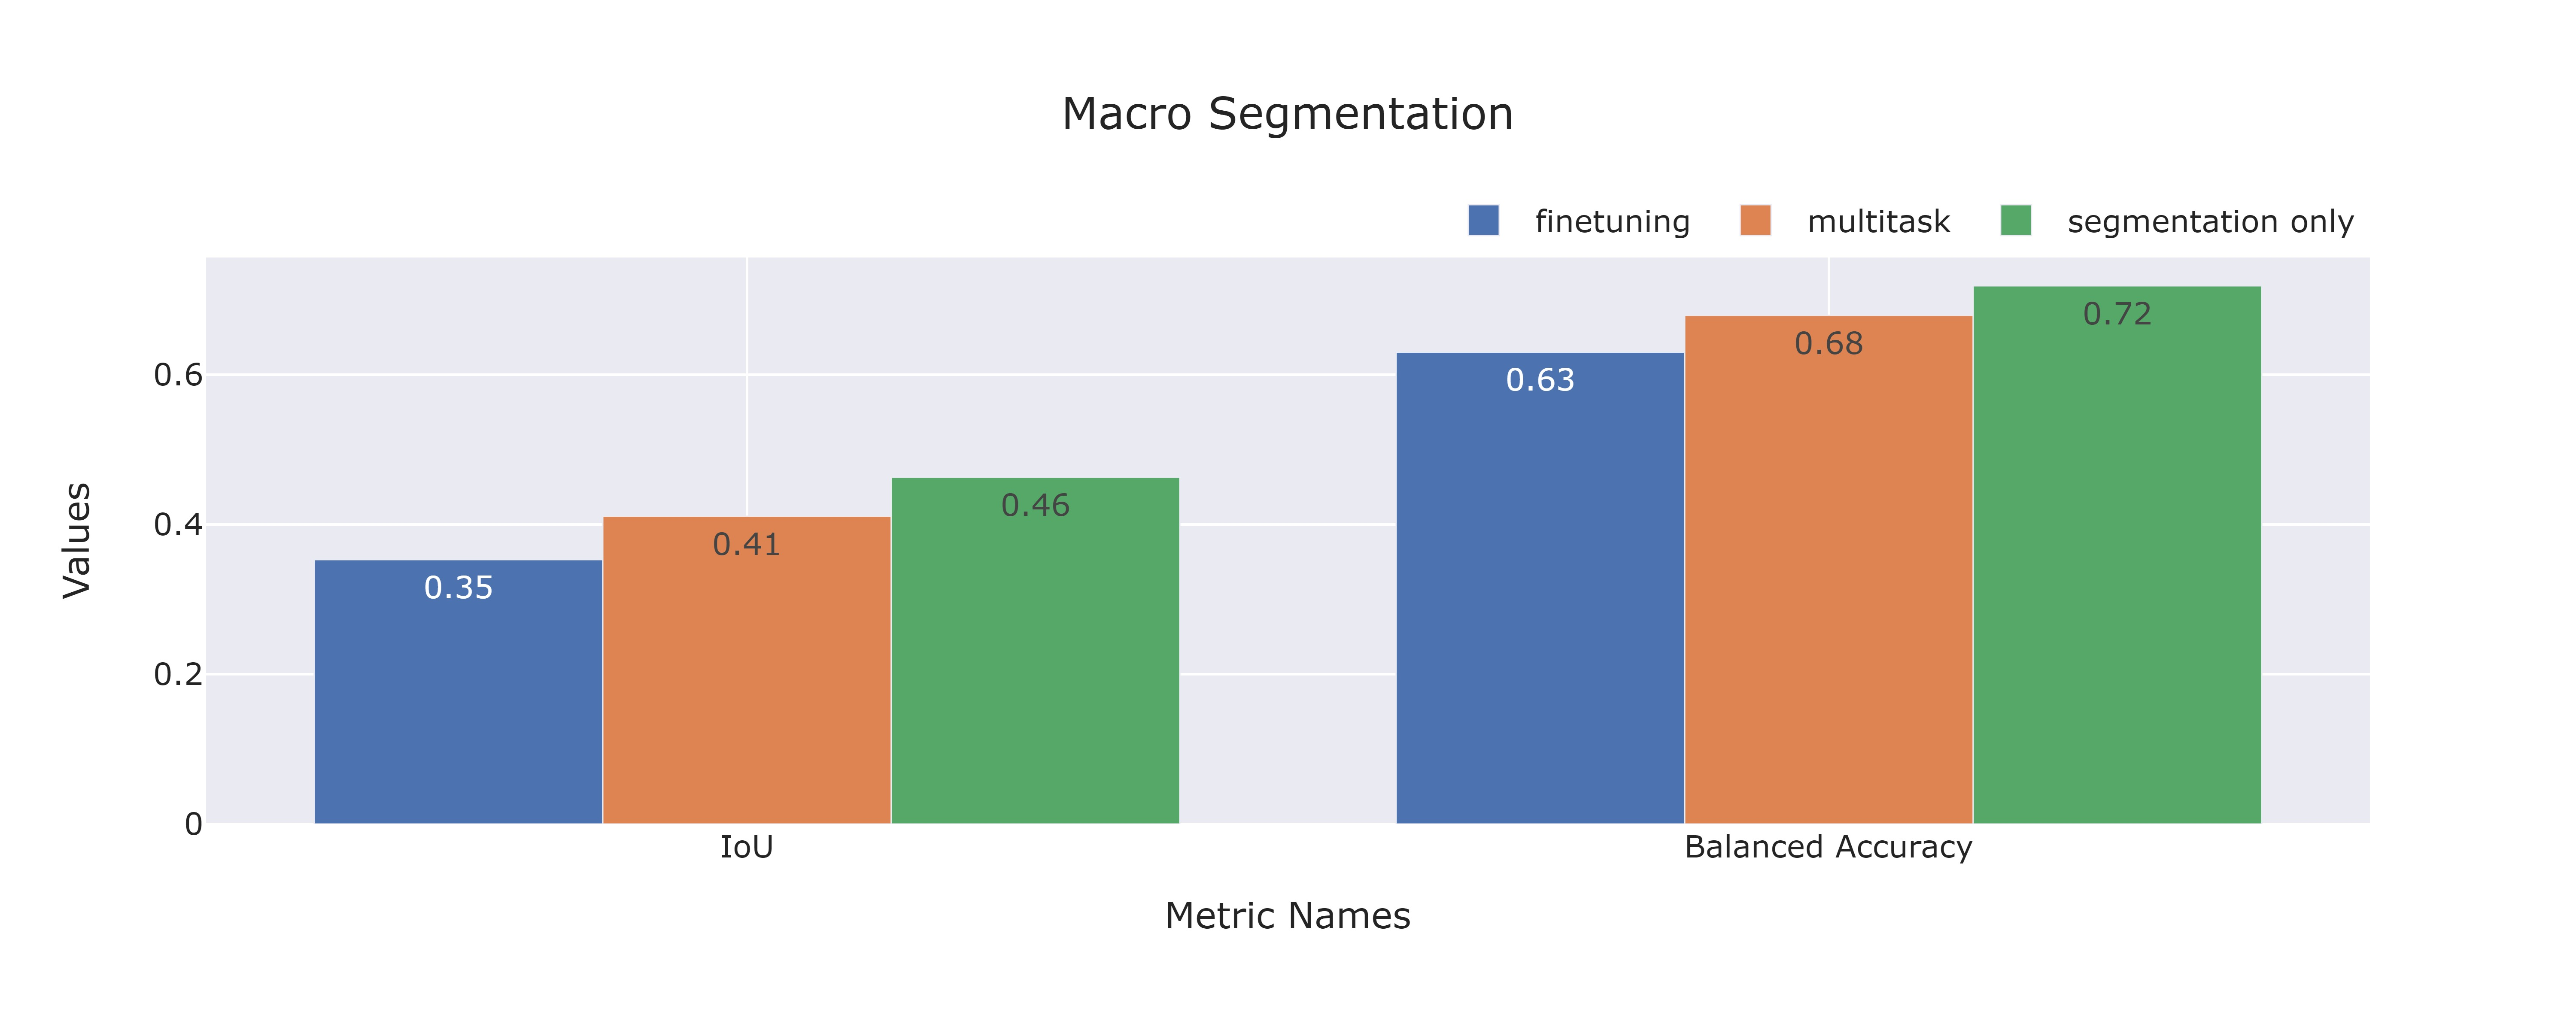
\includegraphics[width=\textwidth]{result_imgs_sorted/Macro-Segmentation.jpeg}
    \caption{Porównanie miar Iou oraz dokładnosci dla segmentacji sceny.}
    \label{fig:macro-segmentation}
\end{figure}

Analizując rysunek \ref{fig:macro-segmentation} nie trudno zauważyć, że najlepsze rezultaty otrzymano w dla uczenia wyłącznie segmentacji. Kolejnym wynikiem jest uczenie wielozadaniowe. Jako najsłabsze podejście okazuje się metoda finetunowania. Relacje jakości są zachowane dla każdej z metryk, a więc zarówno dla miary IoU, jak i zbilansowanej dokładności (bAcc). Widać, że miara IoU wypada gorzej niż bAcc. Wyniki mogą sugerować, że trudno jest przeprowadzić transfer wiedzy z ImageNetu, gdyż finetunowanie wypada najsłabiej. Jest to najprawdopodobniej spowodowane zupełnie innym rozkładem klas dla wspomnianej bazie. Analiza sceny w przeciwieństwie do klasyfikacji najczęściej cechuje się długoogonowym rozkładem klas. Drugim istotnym szczegółem jest fakt, iż wagi dekodera i głowy segmentacyjnej są losowe. Uczenie wielozadaniowe zgodnie z zakładanymi wynikami nie polepsza segmentacji, gdyż łączna przestrzeń segmentacji i klasyfikacji jest niewątpliwie trudniejsza do optymalizacji.

\vspace{0.5cm}
Przechodząc do klasyfikacji, wyróżniamy 5 scenariuszy testowych. Pierwszym jest uczenie wyłącznie klasyfikacji, analogicznie jak wyżej, a więc przy wyłączonej części segmentacyjnej. Kolejnymi są wspomniane wcześniej uczenie wielozadaniowe oraz finetuning. Do nowych scenariuszy zaliczamy bezpośrednią oraz pośrednią klasyfikację z segmentacji.
\begin{figure}[ht!]
    \centering
    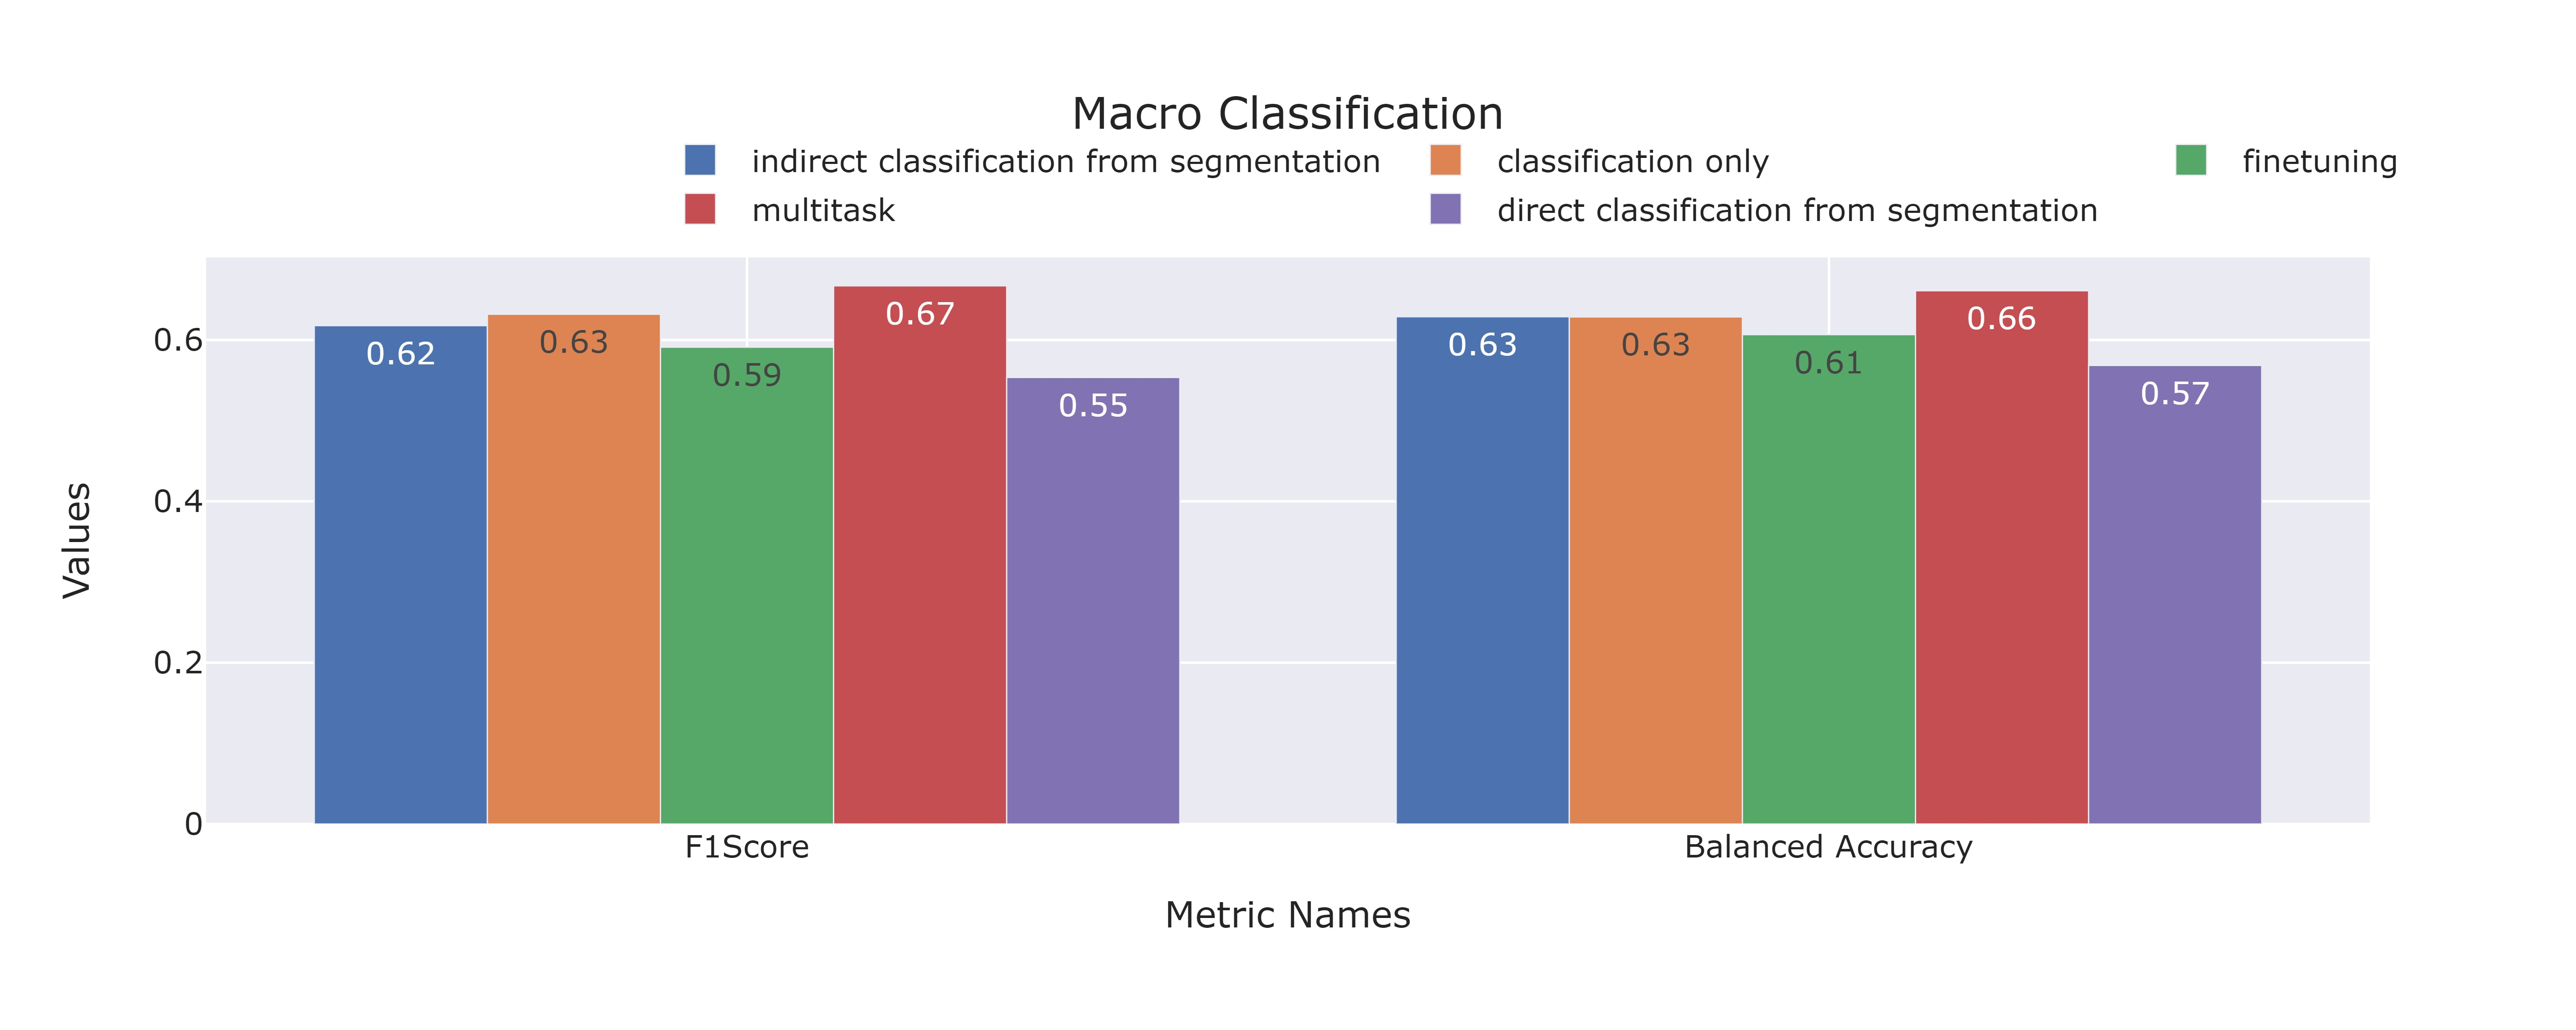
\includegraphics[width=\textwidth]{new/Macro-Classification.jpeg}
    \caption{Porównanie miar F1 oraz dokładnosci dla klasyfikacji sceny.}
    \label{fig:macro-classification}
\end{figure}

Rezultaty przedstawia rysunek \ref{fig:macro-classification}. Od razu da się zauważyć, że wyniki cechuje mniejsze odchylenie standardowe oraz, analizując łącznie miarę F1 oraz zbalansowaną dokładność, średnia. Fakt ten jest prawdopodobnie wynikiem znacznie mniejszej ilości parametrów uczących. Jako najlepszy rezultat uzyskuje uczenie wielozadaniowe. Ciekawym wydaje się fakt, że uczenie wyłącznie klasyfikacji jest słabsze w tym przypadku. Prawdopodobnie poprzez uczenie wielozadaniowe enkoder wygenerował lepszą przestrzeń reprezentacji, co bezpośrednio wpływa na klasyfikację sceny. Najgorszym przypadkiem jest uczenie klasyfikacji bezpośrednio z segmentacji. Nie jest to dziwne, gdyż w tym przypadku klasyfikator korzystał z zaledwie 13 kanałów.
\vspace{0.5cm}

Analizowanie jakości algorytmu dla każdej z klas osobno jest ważne, ponieważ pozwala na bardziej szczegółowe zrozumienie mocnych i słabych stron algorytmu. Rozważając ogólną jakość algorytmu przy użyciu metryki makrośredniej, nie jest od razu jasne, w których klasach algorytm radzi sobie dobrze, a w których źle. Analizując jakość każdej klasy osobno, można zidentyfikować konkretne klasy, z którymi algorytm ma problemy i podjąć kroki w celu poprawy wydajności w tych klasach.

\vspace{0.5cm}
Rysunek \ref{fig:classification-accuracy} przedstawia dokładność dla każdej z klas dla zadania klasyfikacji sceny. Trudno jednoznacznie określić, która z  metod sprawdza się tutaj najlepiej. Uczenie wielozadaniowe wypada najlepiej dla klas: łazienka, sypialnia, salon, biuro. Uczenie wyłącznej klasyfikacji jest najlepsze dla klas jadalnia oraz kuchnia. W pozostałych przypadkach klasa inne pomieszczenia jest najlepiej wykrywana przez scenariusz finetunowania. Uczenie klasyfikacji z segmentacji nigdy nie osiąga najlepszego wyniku.
\begin{figure}[ht!]
    \centering
    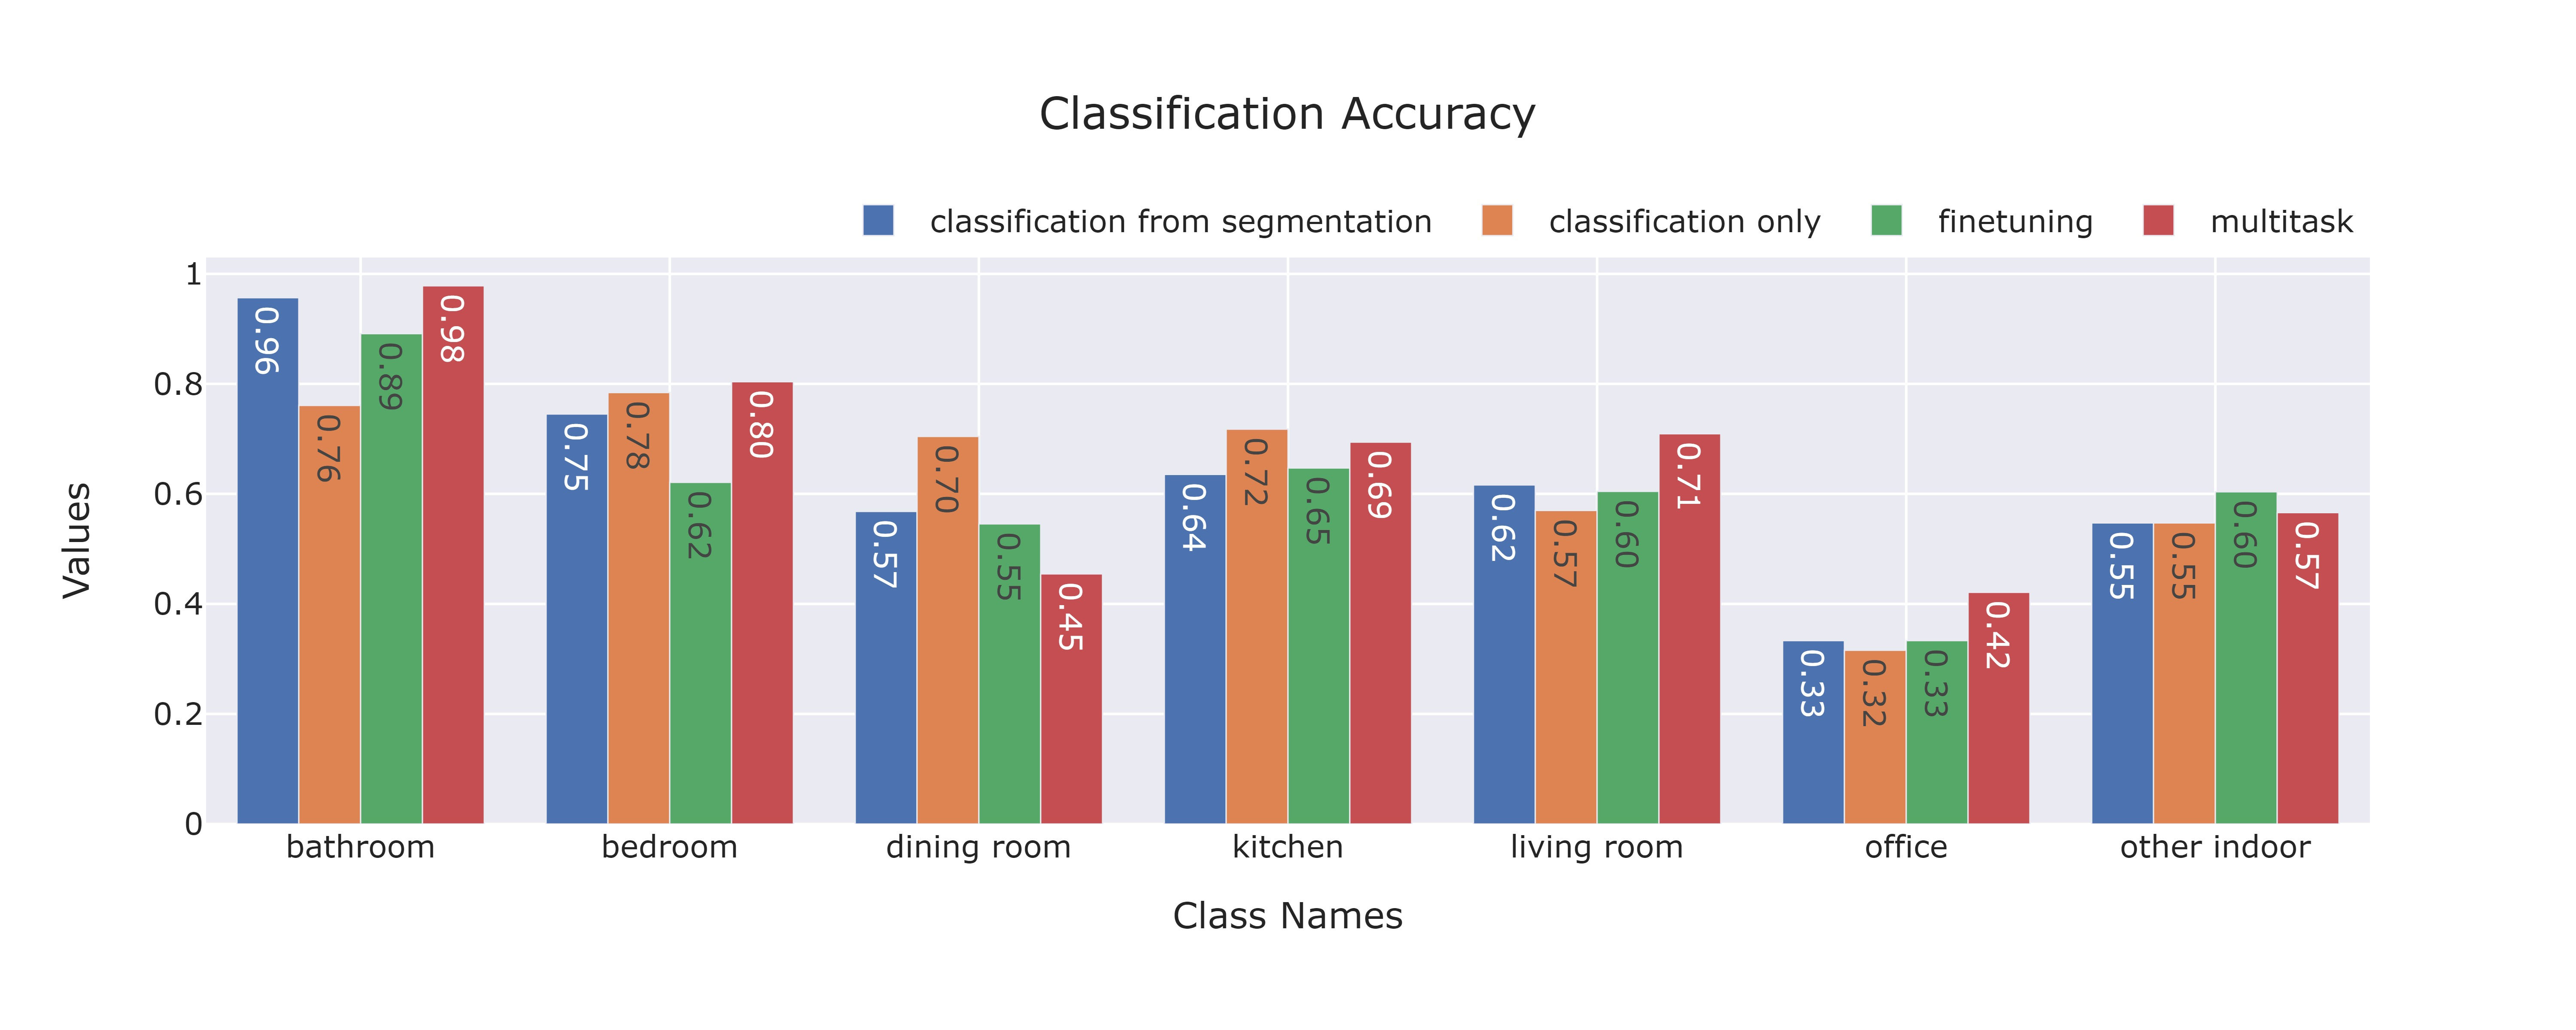
\includegraphics[width=\textwidth]{new/Classification-Accuracy.jpeg}
    \caption{Porównanie dokładności klasyfikacji sceny z rozróżniem konkretnych klas.}
    \label{fig:classification-accuracy}
\end{figure}
Biorąc pod uwagę miarę F1 (rys. \ref{fig:classification-f1}) również nie jesteśmy w stanie wyróżnić faworyzowanej metody. W porównaniu z wcześniej analizowaną dokładnością widać, że uczenie wielozadaniowe utrzymuje w większości przypadku bardzo dobre rezultaty. Widać też, że wyniki w obrębie każdej z klas mało różnią się między sobą.
\begin{figure}[ht!]
    \centering
    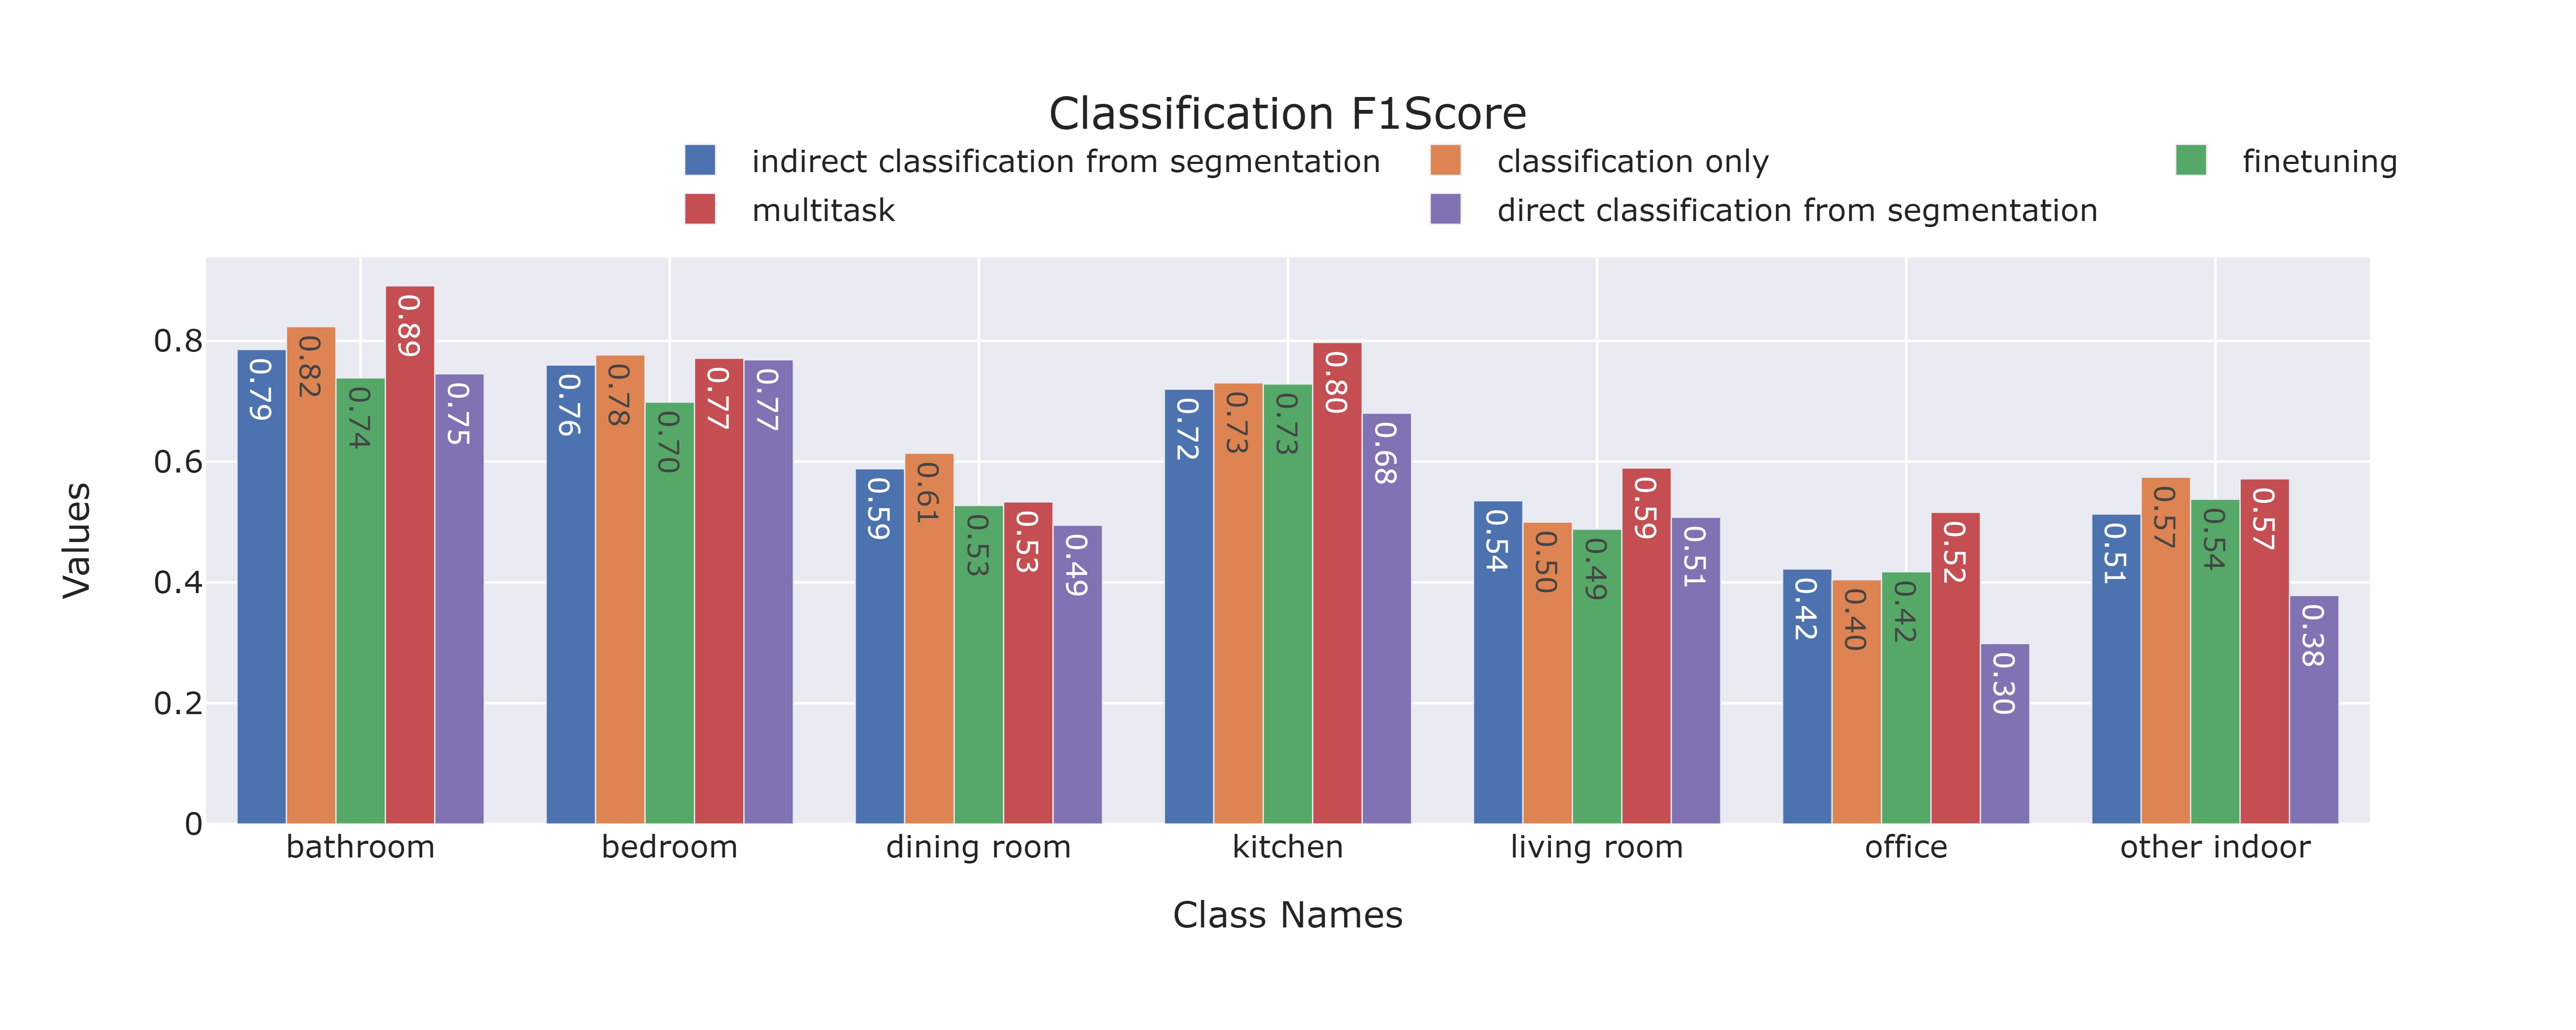
\includegraphics[width=\textwidth]{new/Classification-F1Score.jpeg}
    \caption{Porównanie miary F1 dla klasyfikacji sceny z rozróżniem konkretnych klas.}
    \label{fig:classification-f1}
\end{figure}

\vspace{0.5cm}
Analizując rysunek \ref{fig:segmentation-acc} przestawiający dokładność w zadaniu segmentacji semantycznej, widać, że niektóre z zadań wypadają znacznie gorzej niż pozostałe. Sytuacja ta dotyczy klas meble, stoły, obiekty. Uczenie wyłącznie segmentacji okazało się najlepsze dla klas łóżko, podłoga, meble, obiekty, obraz, tv, ściana oraz okno. Stanowi to ponad połowę wszystkich możliwych klas. Uczenie wielozadaniowe uzyskało najlepsze wyniki dla klas książki, sufit, sofa. Przypadek funetunowania nigdy nie osiągnął najlepszego rezultatu.
\begin{figure}[ht!]
    \centering
    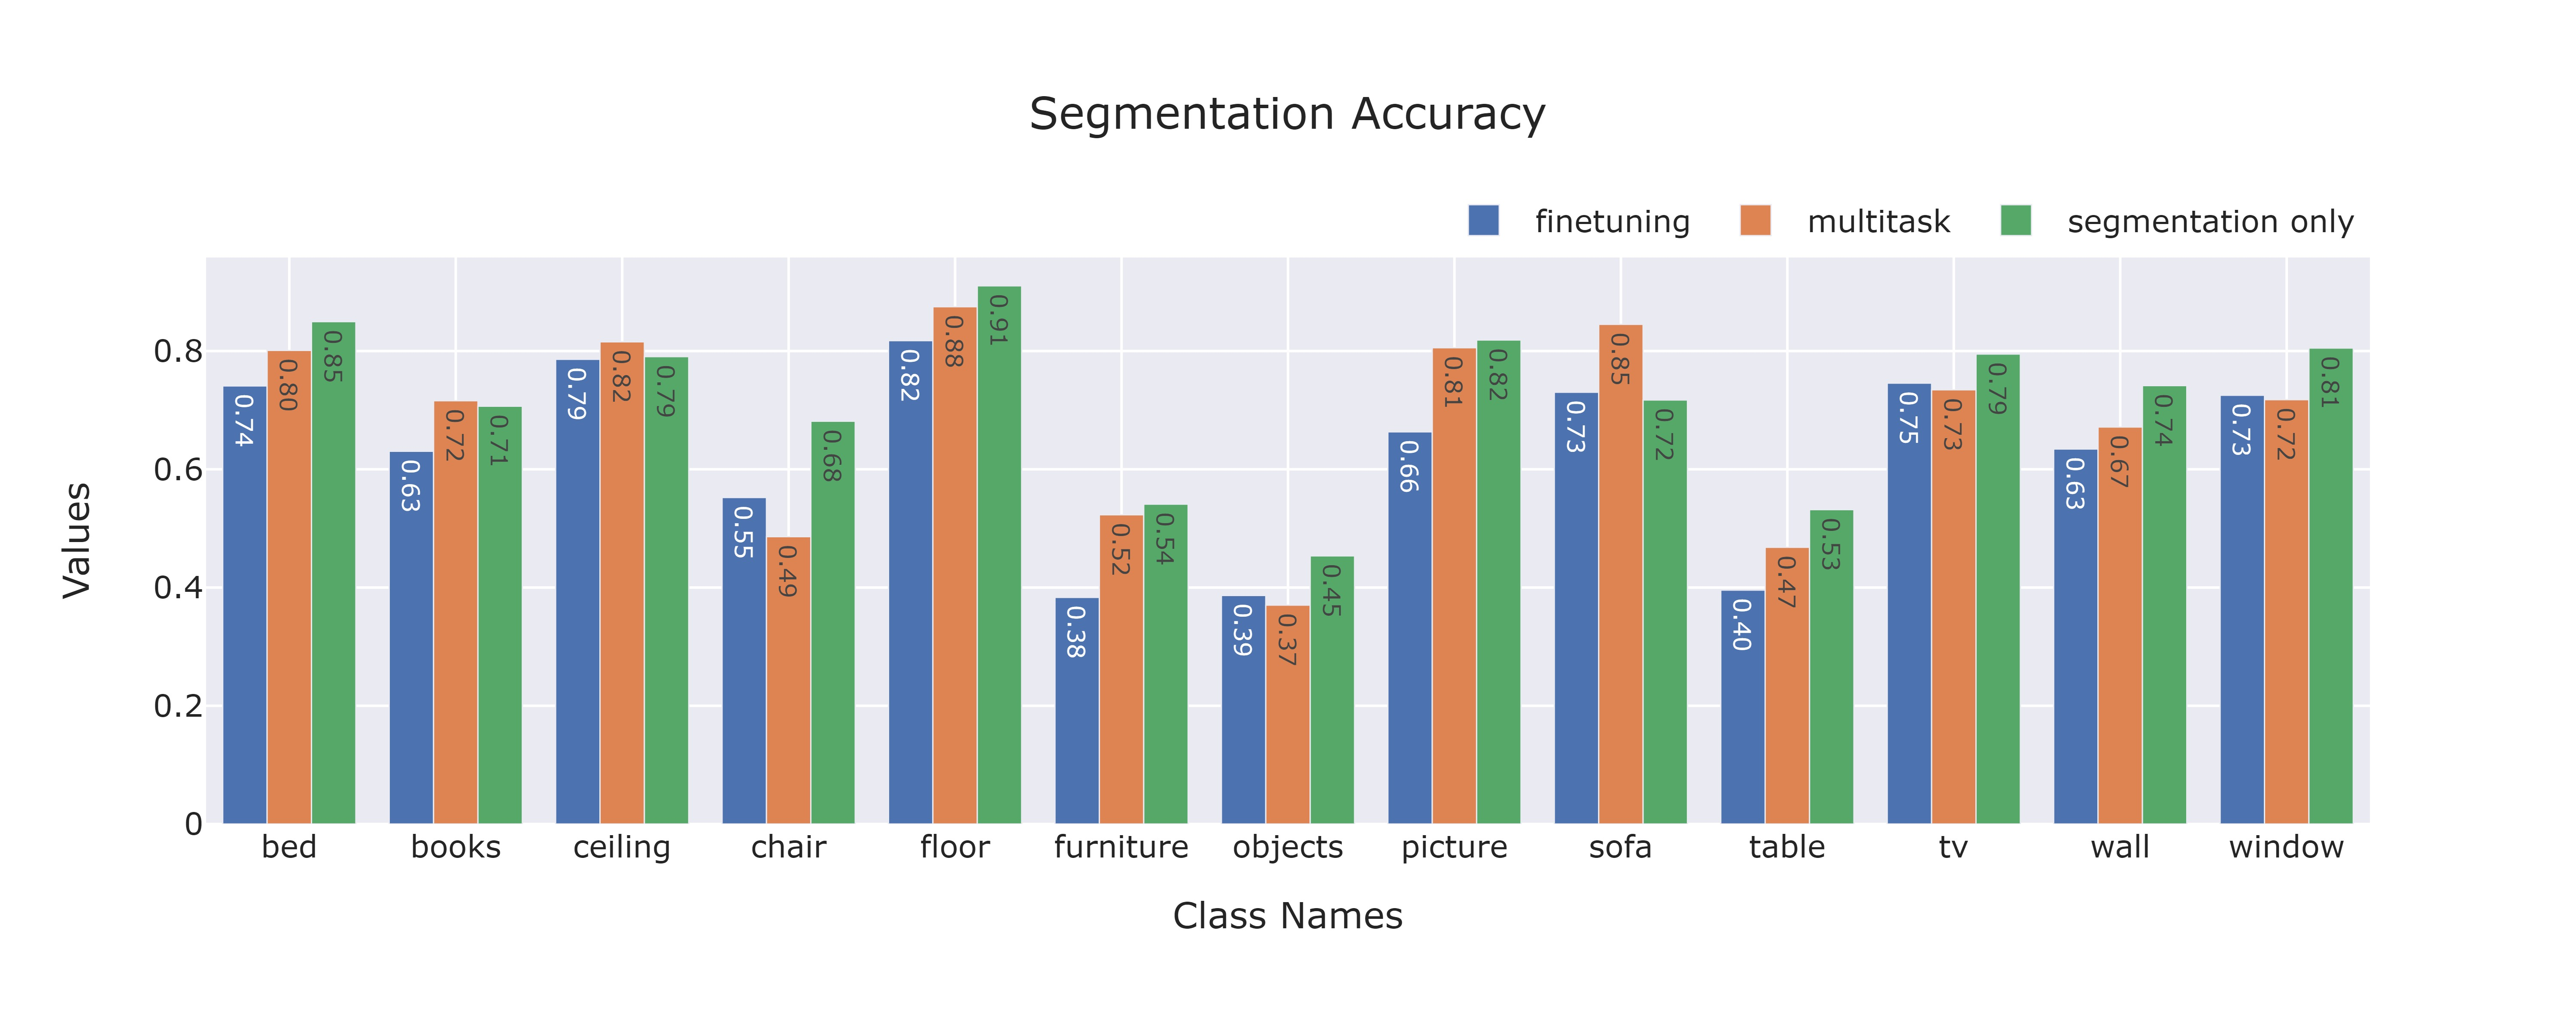
\includegraphics[width=\textwidth]{result_imgs_sorted/Segmentation-Accuracy.jpeg}
    \caption{Porównanie dokładności segmentacji z rozróżniem konkretnych klas.}
    \label{fig:segmentation-acc}
\end{figure}

Na rysunku \ref{fig:segmentation-iou} przestawiono IoU dla segmentacji semantycznej. Widać tutaj dużą dysproporcję między klasami podłoga, ściana, a pozostałymi klasami. Jest to zrozumiałe, klasy te występują stosunkowo często na obrazie. Uczenie wyłącznie segmentacji uzyskuje najlepsze wyniki na wszystkich klasach z wyłączeniem książek oraz telewizorów. W tych przypadkach najlepsze okazuje się uczenie wielozdaniowe.

\begin{figure}[ht!]
    \centering
    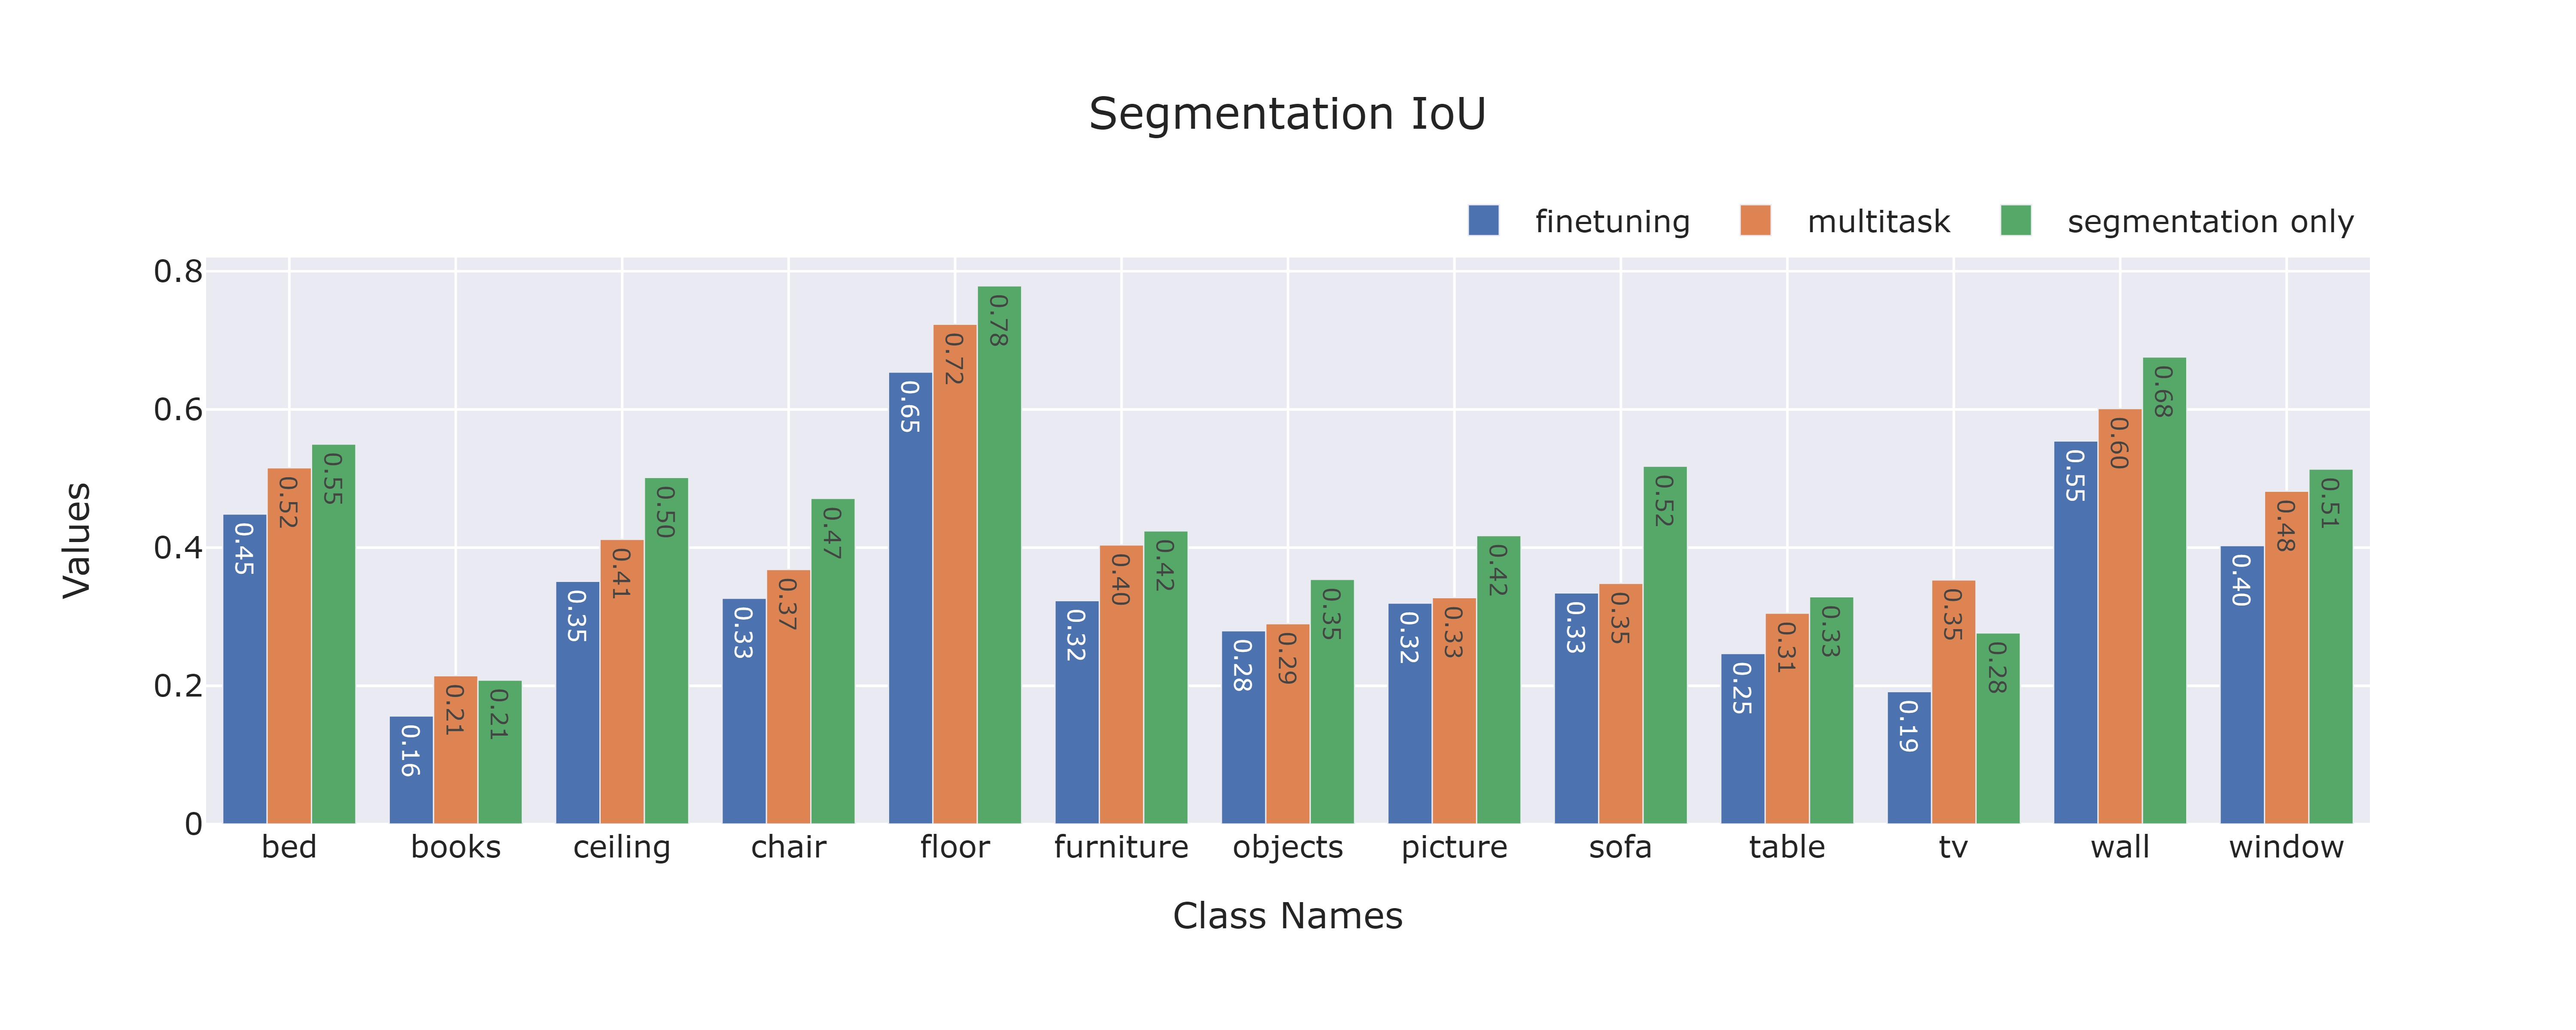
\includegraphics[width=\textwidth]{result_imgs_sorted/Segmentation-IoU.jpeg}
    \caption{Porównanie miary IoU segmentacji z rozróżniem konkretnych klas.}
    \label{fig:segmentation-iou}
    
\end{figure}
\subsection{Analiza czasowa}
Ostatnio coraz częściej mówi się o zapotrzebowaniu na zasoby sprzętowe podczas uczenia maszynowego. Głębokie sieci neuronowe, a szczególnie te przetwarzające obrazy wymagają coraz więcej zasobów obliczeniowych do prawidłowego działania. Wynika to z dwóch głównych czynników. Po pierwsze duże modele wizji komputerowej posiadają miliony parametrów. Drugim powodem jest przetwarzanie wielu obrazów, które de facto są zbiorem macierzy. Wiedzie to do większego zainteresowania zużywanymi zasobami podczas treningu oraz wnioskowania. W tym podrozdziale przedstawiona zostanie analiza czasu treningu oraz wnioskowania.

Analizując czas uczenia w przypadku kolejnych metod, odkrywamy zalety finetuningu oraz uczenia wielozadaniowego (tab. \ref{tab:por-trening-all}). Suma czasów uczenie wyłącznie segmentacji oraz wyłącznie klasyfikacji (około 360s) znacząco przewyższa pozostałe metody. Najbardziej opłacalną czasowo metodą okazuje się finetuning. Jednakże na podstawie wyników miar jakości nie można uznać go za najbardziej optymalny. Pozostają jeszcze dwie metody - nauczenie segmentacji oraz dalsze uczenie klasyfikacji (ok. 260 s . i 275s) oraz uczenie wielozadaniowe (ok. 211s). Segmentacja, a potem klasyfikacja osiąga najlepsze wyniki na segmentacji oraz przeciętne na klasyfikacji. Z drugiej strony uczenie wielozadaniowe osiąga najlepsze rezultaty na klasyfikacji oraz drugi najlepszy wynik na segmentacji. Łącząc to z faktem znacznie krótszego uczenia, można wysunąć wniosek, że uczenie wielozadaniowe jest optymalne pod względem czasu treningu oraz dawanych rezultatów.



% \begin{table}[ht!]
%     \centering
%     \begin{tabular}{c|c}
%         nazwa zadania                      &   czas{[}s{]} \\ \hline
%         wyłącznie segmentacja                  &   188.70 \\
%         wyłącznie klasyfikacja                &   170.47 \\
%         pośrednia klasyfikacja z segmentacji   &   70.78 \\
%         bezpośrednia klasyfikacja z segmentacji   &   88.69 \\
%         finetuning                        &   158.46 \\
%         uczenie wielozadaniowe                   &   210.97 
% \end{tabular}
% \caption{Porównanie czasu uczenia względem metody.}
% \label{tab:acc-por}
% \end{table}


\begin{table}[ht!]
    \centering
    \begin{tabular}{c|c}
        nazwa zadania                      &   czas{[}s{]} \\ \hline
        wyłącznie segmentacja +  wyłącznie klasyfikacja & \textasciitilde 360 \\
        wyłącznie segmetnacja + pośrednia klasyfikacja & \textasciitilde 260 \\
        wyłącznie segmetnacja + bezpośrednia klasyfikacja & \textasciitilde 275 \\
        uczenie wielozadaniowe                   &   \textasciitilde 211 \\
        finetuning                        &   \textasciitilde 160 
\end{tabular}
\caption{Porównanie czasu uczenia względem całości.}
\label{tab:por-trening-all}
\end{table}


Porównanie czasu wnioskowania jest kluczowe z punktu widzenia korzystania z potencjału uczenia maszynowego. Tabela \ref{tab:por-infer} przedstawia zestawienie czasu wnioskowania dla zestawu dwóch szeregowych sieci oraz jednej architektury wykonującej dwa zadania naraz. Pierwszy przypadek obejmuje wykorzystanie wyłącznie klasyfikacji, a następnie wyłącznie segmentacji. W praktyce oznacza to dwukrotne podawanie danych do modelu i przejście przrz 2 razy więcej parametrów niż w pozostałych przypadkach. Rozważając jedną architekturę osiągamy prawie dwukrotnie krótszy czas wnioskowania. Do tego przypadku zaliczamy wszystkie metody z uczeniem klasyfikacji na segmentacji, finetung oraz uczenie wielozadaniowe.


\begin{table}[ht!]
    \centering
    \begin{tabular}{c|c}
        rodzaj sieci                      &   czas{[}s{]} \\ \hline
        dwie szeregowe sieci                  &   15.7\\
        jedna architektura               &   8.6
\end{tabular}
\caption{Porównanie czasu wnioskowania.}
\label{tab:por-infer}
\end{table}

\subsection{Analiza konkretnych przykładów}
Analiza metryk, czy różnych miar jakości jest niezbędna do ewaluacji zadań uczenia maszynowego. Odpowiedni wybór tych miar gwarantuje pełen informacji wgląd, stanowiąc cenny wskazówki ewaluacyjne. Nie mniej nie wyklucza to istoty sprawdzenia rezultatów przez ludzkie oko. Mimo że trudno byłoby przeglądać i ewaluować wiele zdjęć w dużych zbiorach danych, przekrojowe sprawdzenie jest kluczowe w analizie. Dostarcza bowiem wielu cennych, nieujętych w matematycznych formułach obserwacji. W tym podrozdziale przedstawione zostaną rezultaty na wybranych zdjęciach.
\subsubsection{Segmentacja semantyczna}
Segmentacja semantyczna jest zadaniem niewątpliwie trudnym. Jednocześnie równie ciężko jest określić dobrą funkcję jakości, uwzględniającą takie właściwości jak gładkość, dokładność czy precyzja segmentacji. Można oczywiście korzystać z wielu funkcji jakości, jednak ostateczny werdykt warto przejrzeć ręcznie. W połączeniu z wiedzą dotyczącą między innymi trudności klasyfikacji danej grupy pikseli lub niejedoznacznością niektórych grup pikseli po obejrzeniu nawet kilkunastu zdjęć jesteśmy w stanie wykuć pewne wnioski.

\noindent
\textbf{Łazienka}

Analizując rysunek \ref{fig:bathroom-pred-1} widzimy, że klasa przedmioty (ang. objects) jest bardzo szeroko rozumiana przez twórców zbioru danych. Wynika z tego fakt, że grupa ta nie posiada ściśle określonych cech, które byłyby łatwo identyfikowalne. Model w tym przypadku połączył w sposób szeroki omawianą klasę. Ciekawą obserwacją jest zaznaczenie przez model klasy krzesło. Po głębszej analizie można przypuszczać, że zlew ma podobna teksturę oraz kształt to metalowego krzesła. Klasy ściana, podłoga oraz meble została dość precyzyjnie sklasyfikowana.

\begin{figure}[ht!]
    \centering
    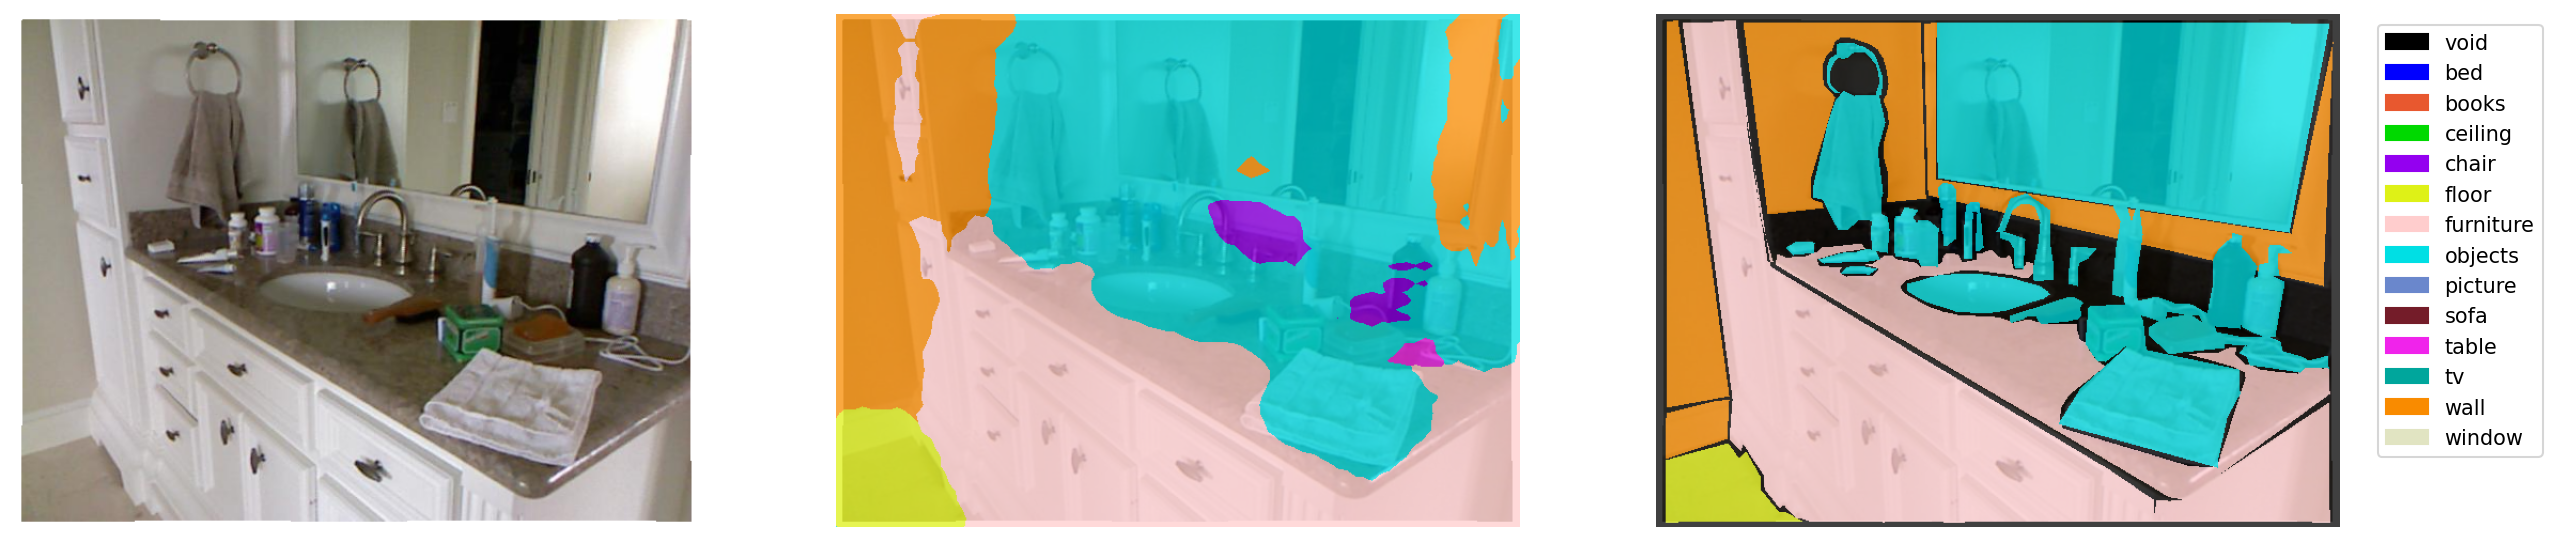
\includegraphics[width=\textwidth]{img/preds_analysis/gt_vs_pred/bathroom-1.png}
    \caption{Porównanie jakości segmentacji dla klasy łazienka.}
    \label{fig:bathroom-pred-1}
\end{figure}

Sytuacja jest równie interesująca w przypadku rysunku \ref{fig:bathroom-pred-2}. Model dopatruje się klasy meble w okolicach drzwi oraz przy zlewie. Pierwszy przypadek jest całkiem zrozumiały. Drewniane drzwi co do faktury mogą przypominać meble, na przykład drzwi od szafki. W drugiej sytuacji można domniemywać, że meble były często związane z umywalką czy nawet zlewem kuchennym, stąd model chętnie te klasy przydziela. Interesujące jest przydzielenie przez model etykiety obraz do włącznika światła.

\begin{figure}[ht!]
    \centering
    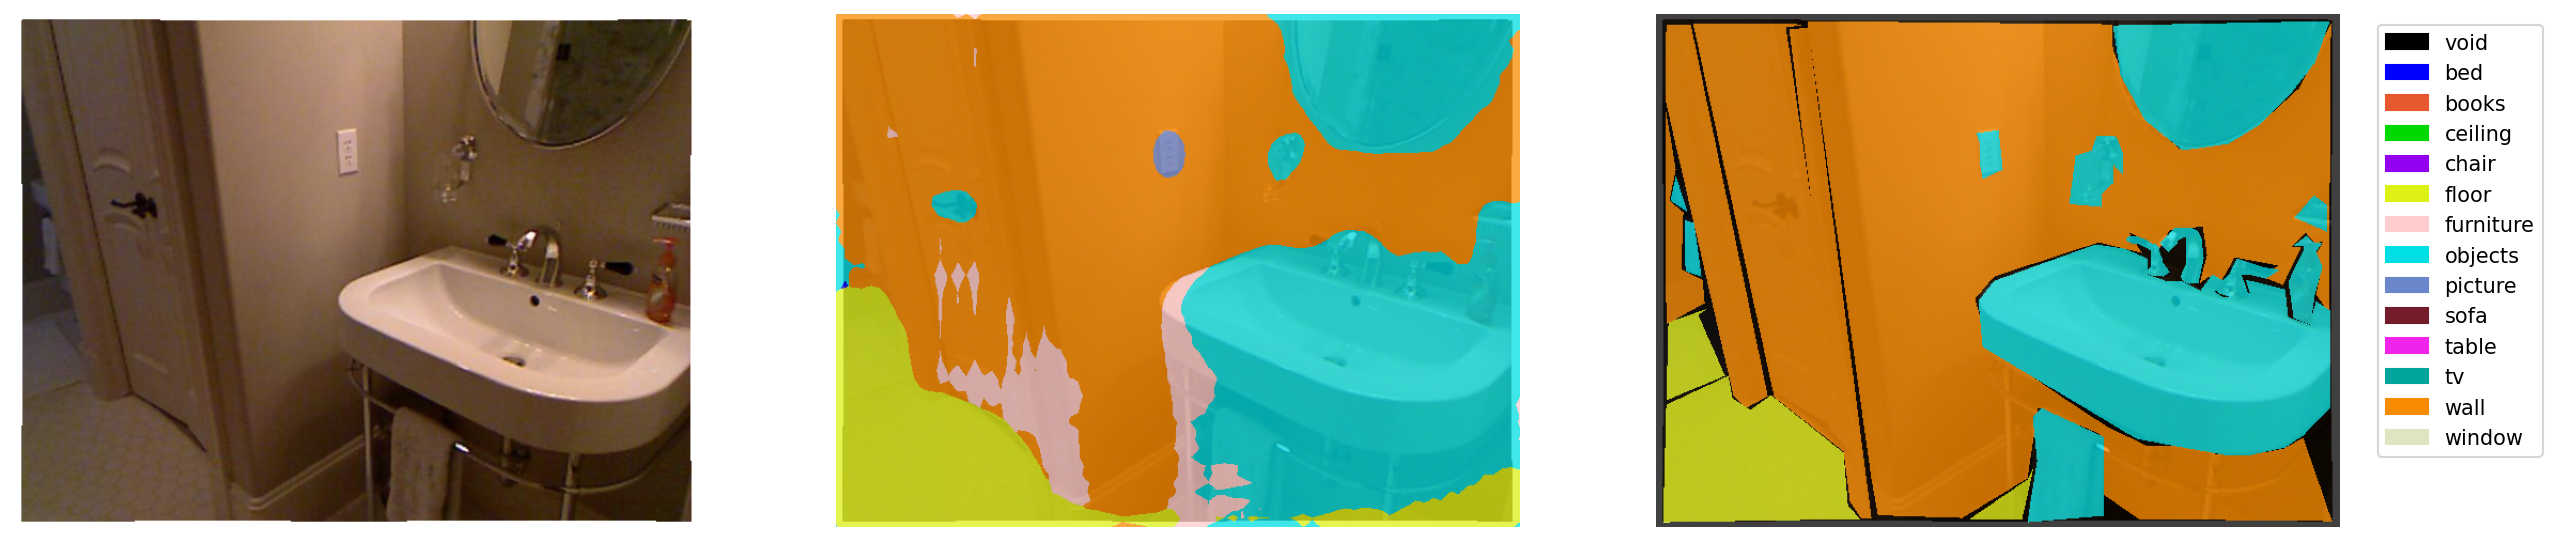
\includegraphics[width=\textwidth]{img/preds_analysis/gt_vs_pred/bathroom-2.png}
    \caption{Porównanie jakości segmentacji dla klasy łazienka.}
    \label{fig:bathroom-pred-2}
\end{figure}

Ostatnim obraz, przedstawiający łazienkę pokazuje rysunek \ref{fig:bathroom-pred-3}. Tak jak wcześniej wspomniano ściany oraz podłoga są często dobrze klasyfikowane. Tak też jest w tym przypadku. Kosz na pranie okazał się wyzwaniem. Model doszukiwał się tu takich obiektów jak stół, krzesło czy mebel.

\begin{figure}[ht!]
    \centering
    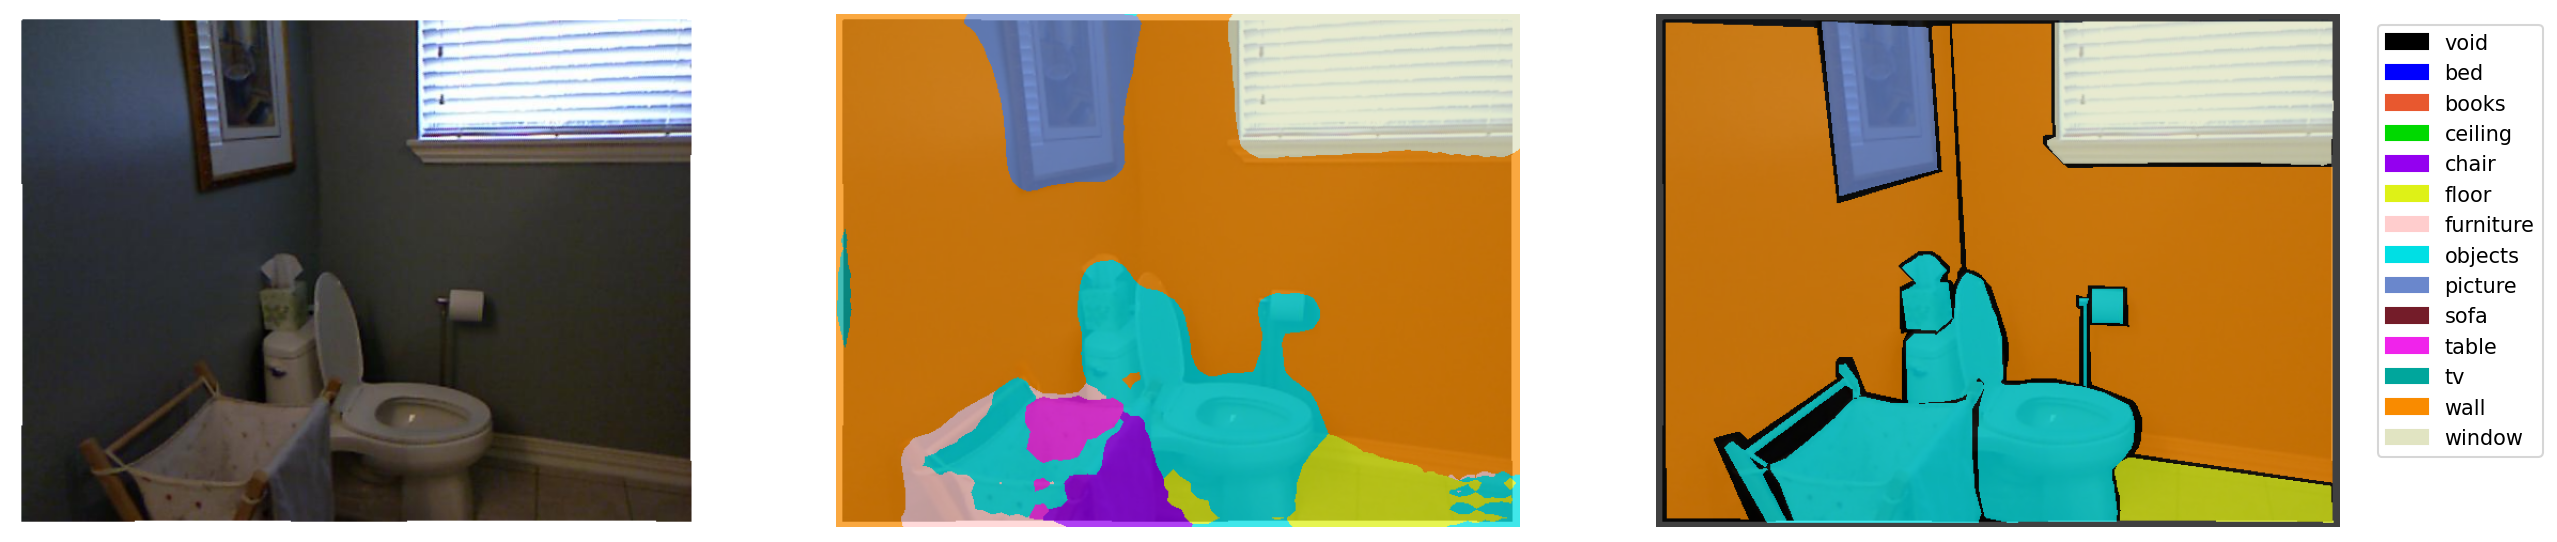
\includegraphics[width=\textwidth]{img/preds_analysis/gt_vs_pred/bathroom-3.png}
    \caption{Porównanie jakości segmentacji dla klasy łazienka.}
    \label{fig:bathroom-pred-3}
\end{figure}

\noindent
\textbf{Salon}

Salon jest najczęściej reprezentowany przez duży pokój, w którym znajdują się kanapa, stolik z przedmiotami, krzesła/fotele oraz ściany z zawieszonymi obrazkami. Nie brakuje tutaj mebli i wielu obiektów.

Rysunek \ref{fig:living_room-pred-1} jest przykładem częstego problemu adnotacji zdjęć. Często okazuje się, że dana grupa pikseli przedstawia więcej niż jedną klasę. Obraz oczekiwany przedstawia regał z książkami jako mebel. Model stwierdził jednak wcale się nie myląc, że są to książki. Trudno się nie zgodzić z tą predykcją. Oznacza to, że zbiór jest poniekąd wewnętrznie sprzeczny w jakiejś części. Widać, że częstym kłopotem jest odróżnienie mebli od stołu. Zadowala fakt pierwszoplanowej kanapy, która bez poduszek została bardzo dobrze sklasyfikowana. Równie dobre rezultaty otrzymujemy dla klasy podłoga, sufit oraz obrazy. Dziwi natomiast fakt zaznaczenia fotela jako krzesła.

\begin{figure}[ht!]
    \centering
    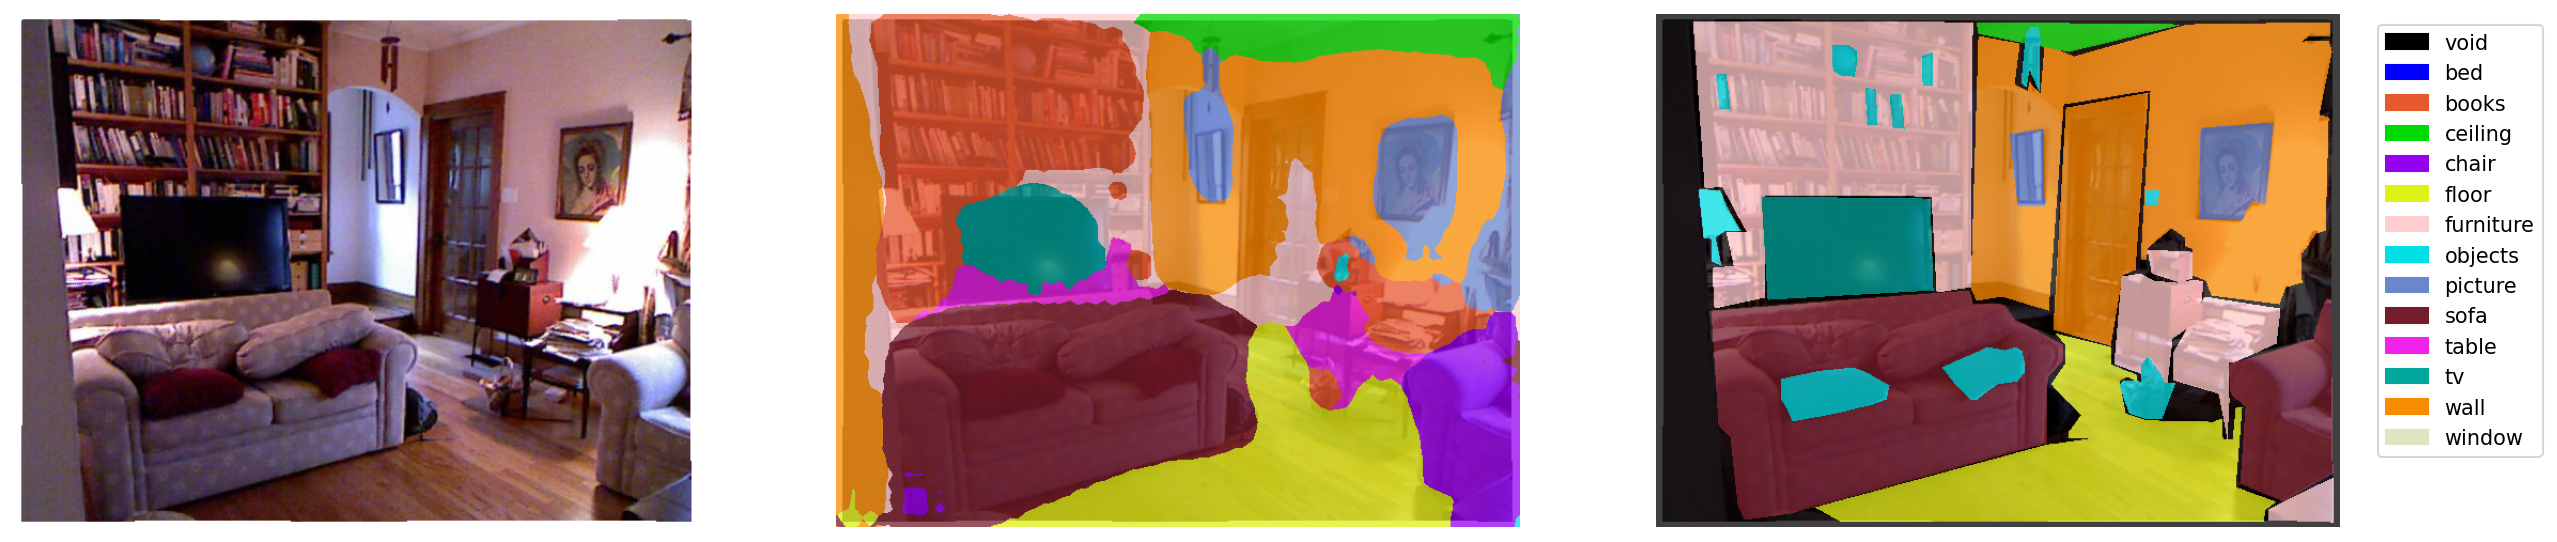
\includegraphics[width=\textwidth]{img/preds_analysis/gt_vs_pred/living_room-1.png}
    \caption{Porównanie jakości segmentacji dla klasy salon.}
    \label{fig:living_room-pred-1}
\end{figure}

Na kolejnym rysunku \ref{fig:living_room-pred-2} sytuacja jest nieco gorsza. Model miał trudności ze wskazaniem stolika na środku, który klasyfikuje jako część kanapy. Sporo problemów wygenerowała klasa krzesło. Obrazy, ściany i podłoga zostały poprawnie sklasyfikowane. Przedmioty drugoplanowe, szczególnie dalsze, a więc mniejsze pozostały dla modelu jednakie.
\begin{figure}[ht!]
    \centering
    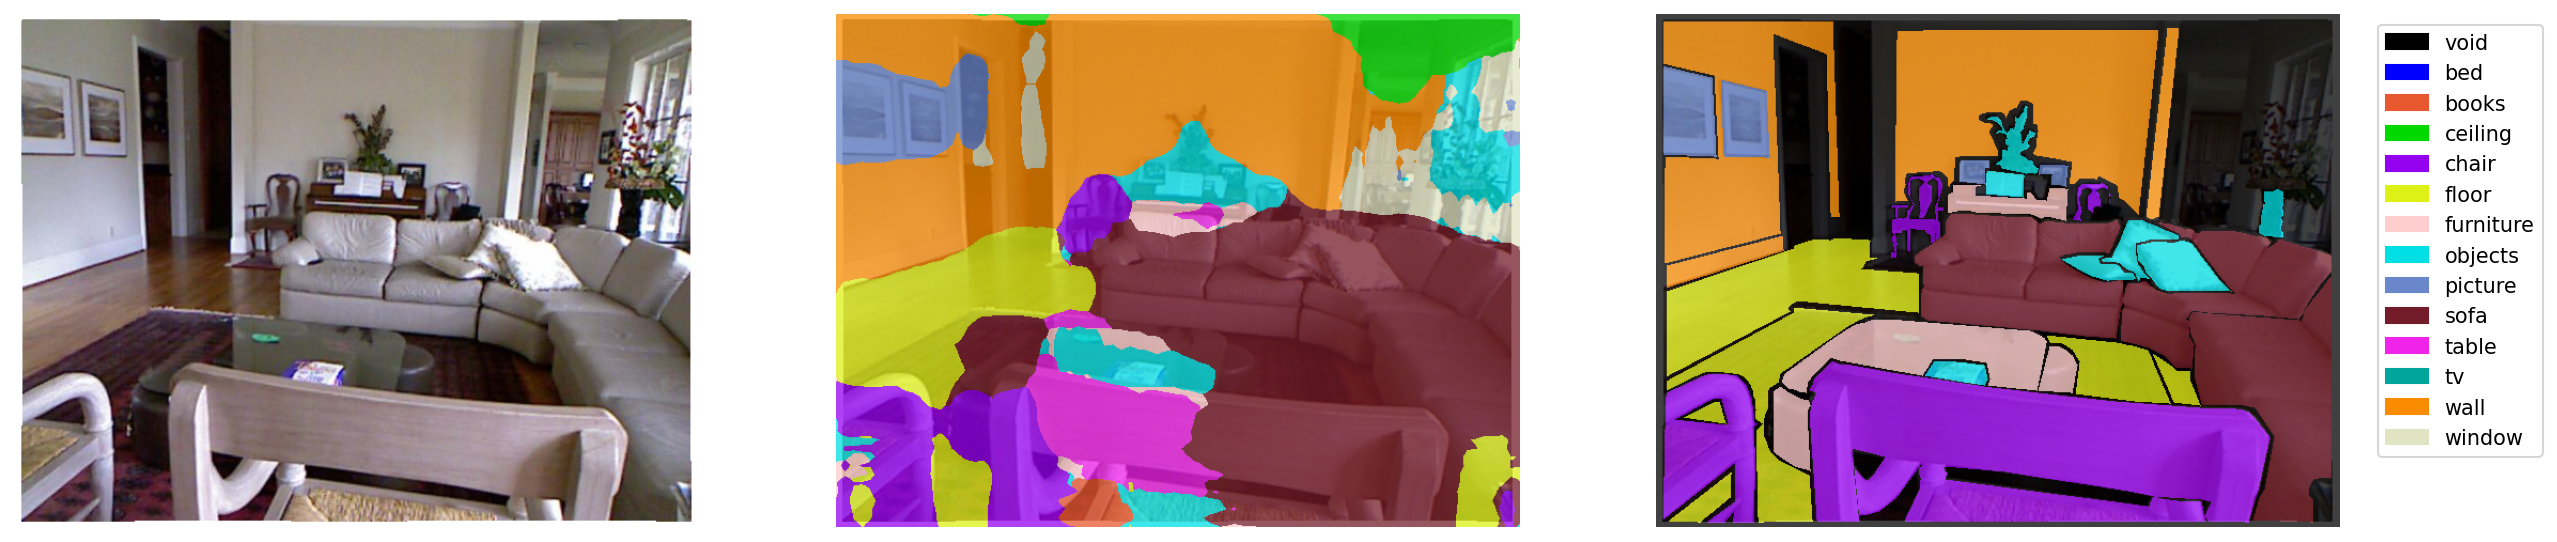
\includegraphics[width=\textwidth]{img/preds_analysis/gt_vs_pred/living_room-2.png}
    \caption{Porównanie jakości segmentacji dla klasy salon.}
    \label{fig:living_room-pred-2}
\end{figure}

Scena salonu (rys. \ref{fig:living_room-pred-3}) jest znacznie lepiej sklasyfikowana niż poprzednia. Oprócz całkiem dobrze sklasyfikowanego stołu, obiektów i kanapy jest jeden ciekawy aspekt. Mianowicie obrazy docelowe znajdujące sie w głąb obrazu zostały pominięte, czyli przedstawione jako pusta (ang. void). Mimo to klasyfikator celnie nadaje im klasy ściana oraz okna. To bardzo dobry prognostyk.

\begin{figure}[ht!]
    \centering
    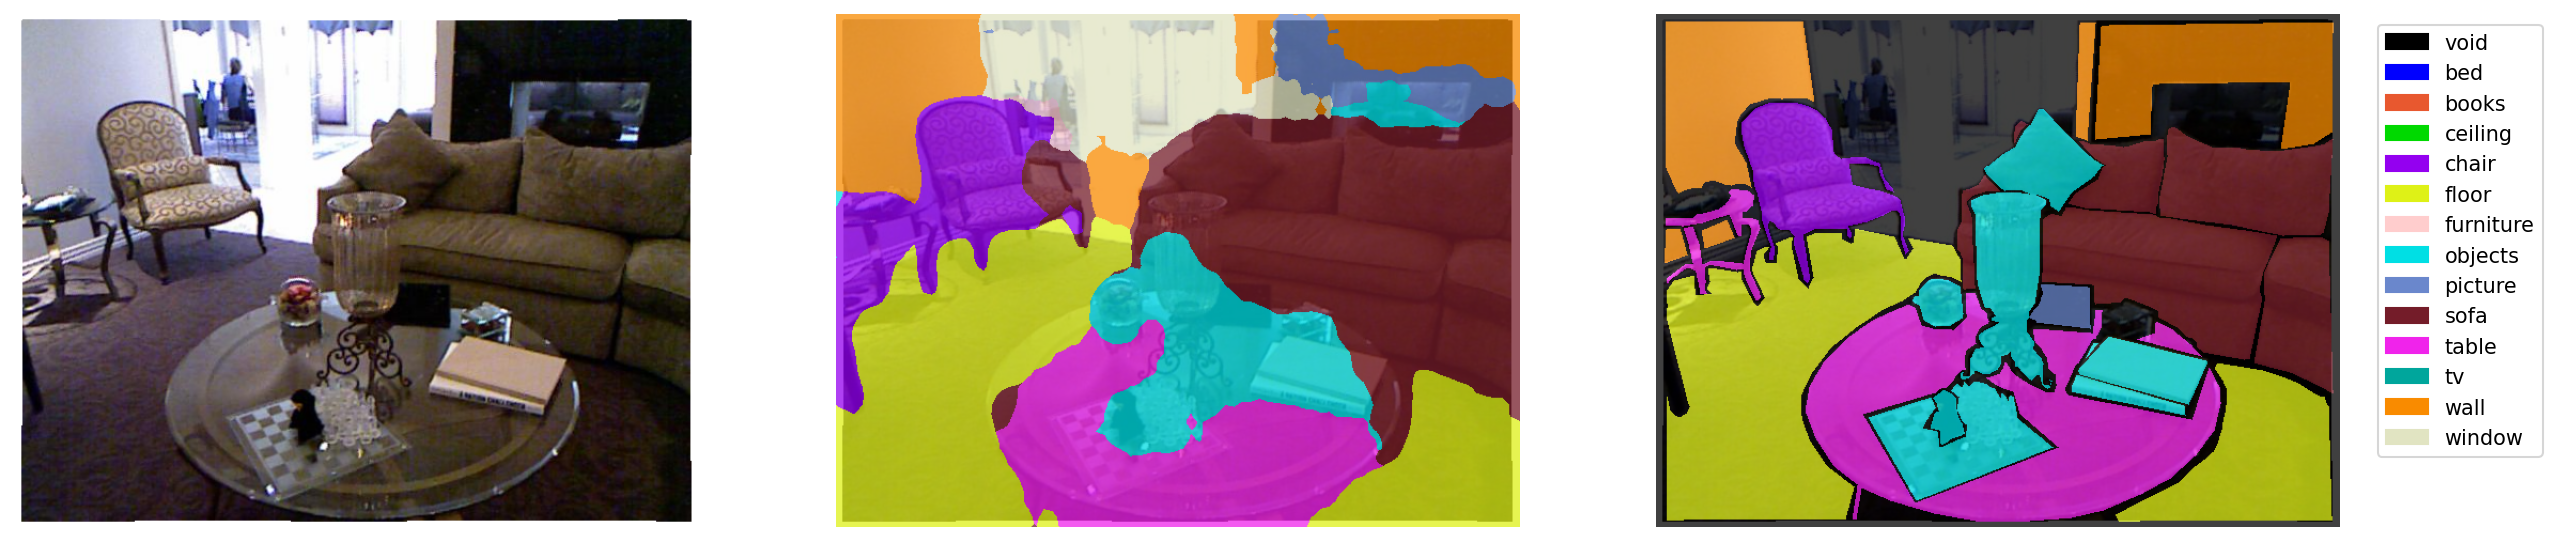
\includegraphics[width=\textwidth]{img/preds_analysis/gt_vs_pred/living_room-3.png}
    \caption{Porównanie jakości segmentacji dla klasy salon.}
    \label{fig:living_room-pred-3}
\end{figure}

\noindent
\textbf{Sypialnia}

Sypialnia to miejsce bardzo złożone. Jednak do charakterystycznych punktów tej sceny należą: łóżko, krzesło, meble oraz okno. Pożądanym byłoby zatem osiągać na tych klasach satysfakcjonujące rezultaty. Na pierwszym planie rysunku \ref{fig:bedroom-pred-1} wdać krzesło, stół oraz szafkę, które w przybliżeniu zostały całkiem dobrze sklasyfikowane. Brak zastrzeżeń budzą również klasy łóżko, podłoga oraz obiekty. Niewątpliwe ciekawe jest poprawne zaznaczenie okna, nawet w porze nocy. Jest to szczególnie cenna informacja, bo czarny prostokąt mógłby być zaklasyfikowany jako na przykład telewizor. Okno zostało zaznaczone zbyt szeroko, mianowicie fałszywie uznając prawdopodobnie lampę za okno. Prawdopodobnie kolor miał tu duże znaczenie.

\begin{figure}[ht!]
    \centering
    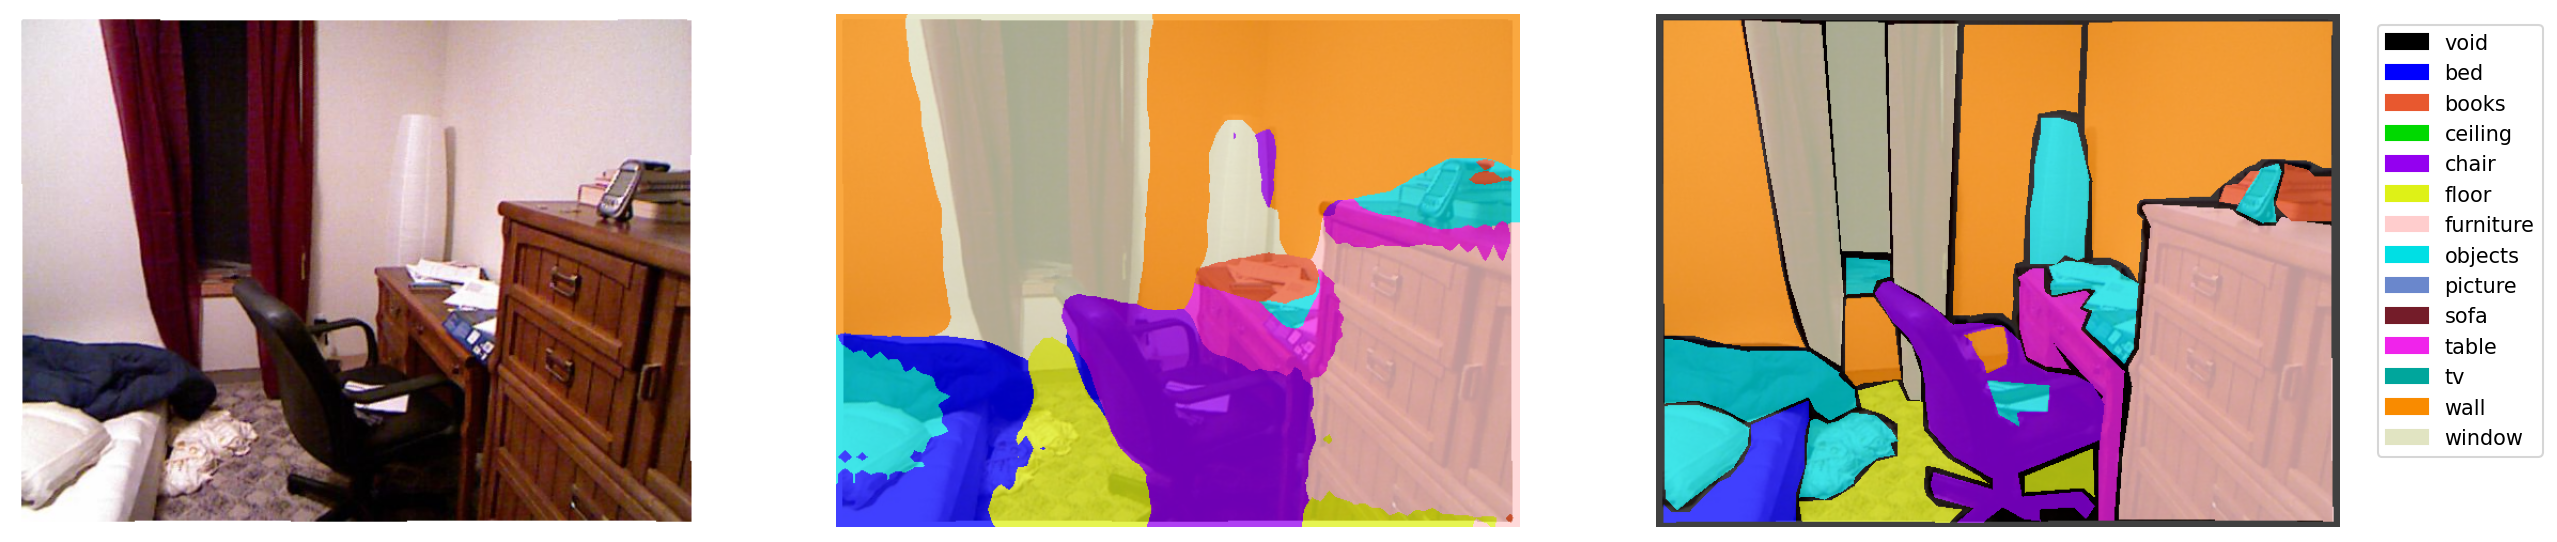
\includegraphics[width=\textwidth]{img/preds_analysis/gt_vs_pred/bedroom-1.png}
    \caption{Porównanie jakości segmentacji dla klasy sypialnia.}
    \label{fig:bedroom-pred-1}
\end{figure}

Rysunek \ref{fig:bedroom-pred-2} to typowe zdjęcie sypialni. Czarną ramę łóżka model uznał za telewizor. Gdyby wyciąć samą tę ramę, wybór rzeczywiście nie byłby oczywisty. Poza tym łózko zostało oznaczone całkiem poprawnie. Dziwi fakty sufitu w miejscu ściany, dla maski docelowej. Model słusznie przypisał tam ścianę. Obrazy zostały poprawnie oznaczone. Na zdjęciu widać, całkiem poprawną próbę klasyfikacji krzesła.

\begin{figure}[ht!]
    \centering
    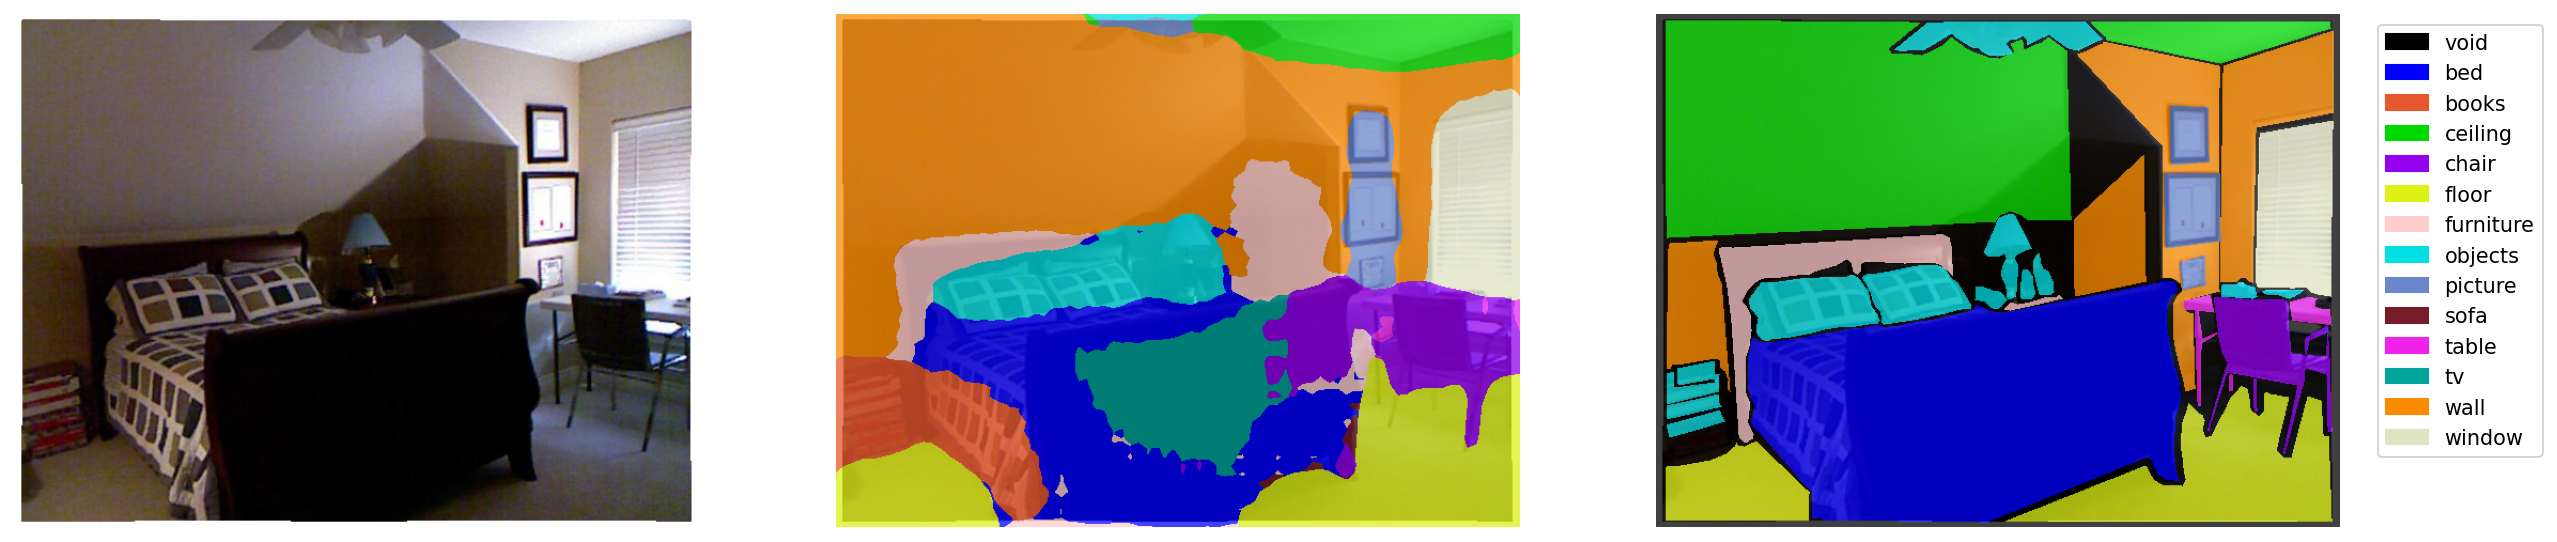
\includegraphics[width=\textwidth]{img/preds_analysis/gt_vs_pred/bedroom-2.png}
    \caption{Porównanie jakości segmentacji dla klasy sypialnia.}
    \label{fig:bedroom-pred-2}
\end{figure}

Ostatni rysunek (rys. \ref{fig:bedroom-pred-3}) był większym wyzwaniem dla modelu. Widać to szczególnie w przypadku pierwszoplanowego biurka. Model nie był w stanie podjąć decyzji co do ostatecznej klasy. Standardowo podłoga oraz sufit zostały sklasyfikowane prawidłowo. Nie inaczej było w przypadku klasy łózko.
\begin{figure}[ht!]
    \centering
    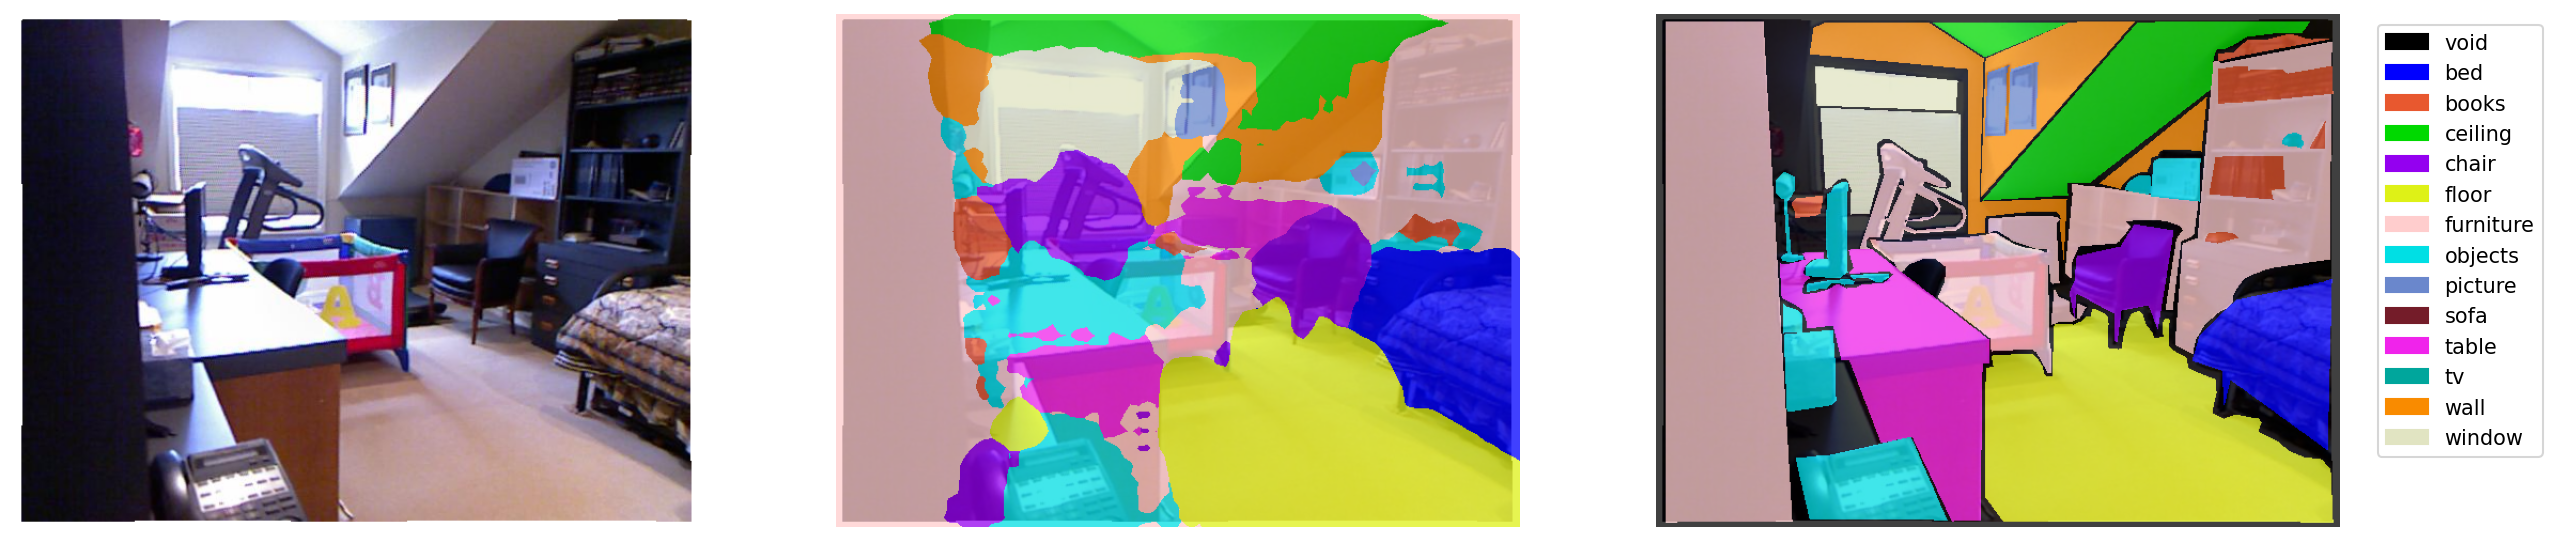
\includegraphics[width=\textwidth]{img/preds_analysis/gt_vs_pred/bedroom-3.png}
    \caption{Porównanie jakości segmentacji dla klasy sypialnia.}
    \label{fig:bedroom-pred-3}
\end{figure}

\noindent
\textbf{Jadalnia}


Obrazy związane z jadalnią to głównie sceny związane ze stołami oraz krzesłami.

Taka sytuacja ma też miejsce na rysunku \ref{fig:dining_room-pred-1}. Właściwie trudno tutaj znaleźć coś szczególnie interesującego. Cały obraz został całkiem dobrze pogrupowany. Wątpliwości budzi jedynie przypisanie do żyrandola klasy obrazy. Prawdopodobnie obrazy znajdujące się obok miały na to wpływ.


\begin{figure}[ht!]
    \centering
    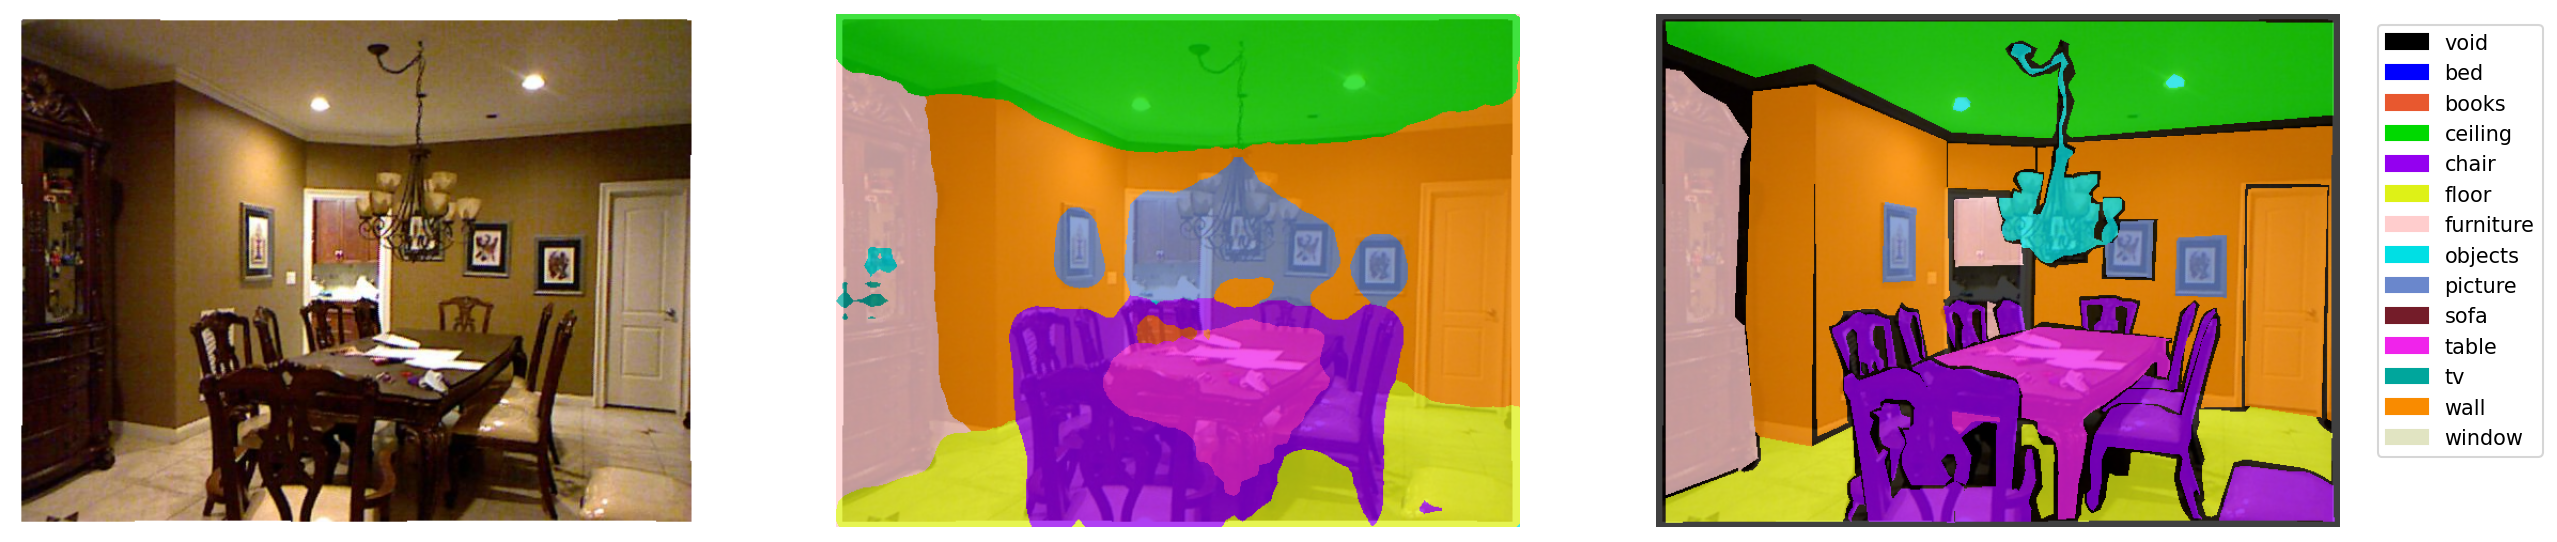
\includegraphics[width=\textwidth]{img/preds_analysis/gt_vs_pred/dining_room-1.png}
    \caption{Porównanie jakości segmentacji dla klasy jadalnia.}
    \label{fig:dining_room-pred-1}
\end{figure}

Przypadek rysunku \ref{fig:dining_room-pred-2} wydaje się ciekawszym. Szczególnie warte uwagi są tutaj okna, na których znajdują się odbicia lustrzane. Refleksy są w wizji komputerowej zagadnieniem od dawna poruszanym i znanym. Można jednoznacznie stwierdzić, że trudno sobie poradzić w takich sytuacjach. Model prawdopodobnie mając trudności z tym obszarem, przypisał go do klasy obiekt. Oprócz tego widzimy problemy z krzesłami w prawym dolnym rogu. Jasna, połyskująca skóra rzeczywiście przypomina nieco płytki podłogowe.

\begin{figure}[ht!]
    \centering
    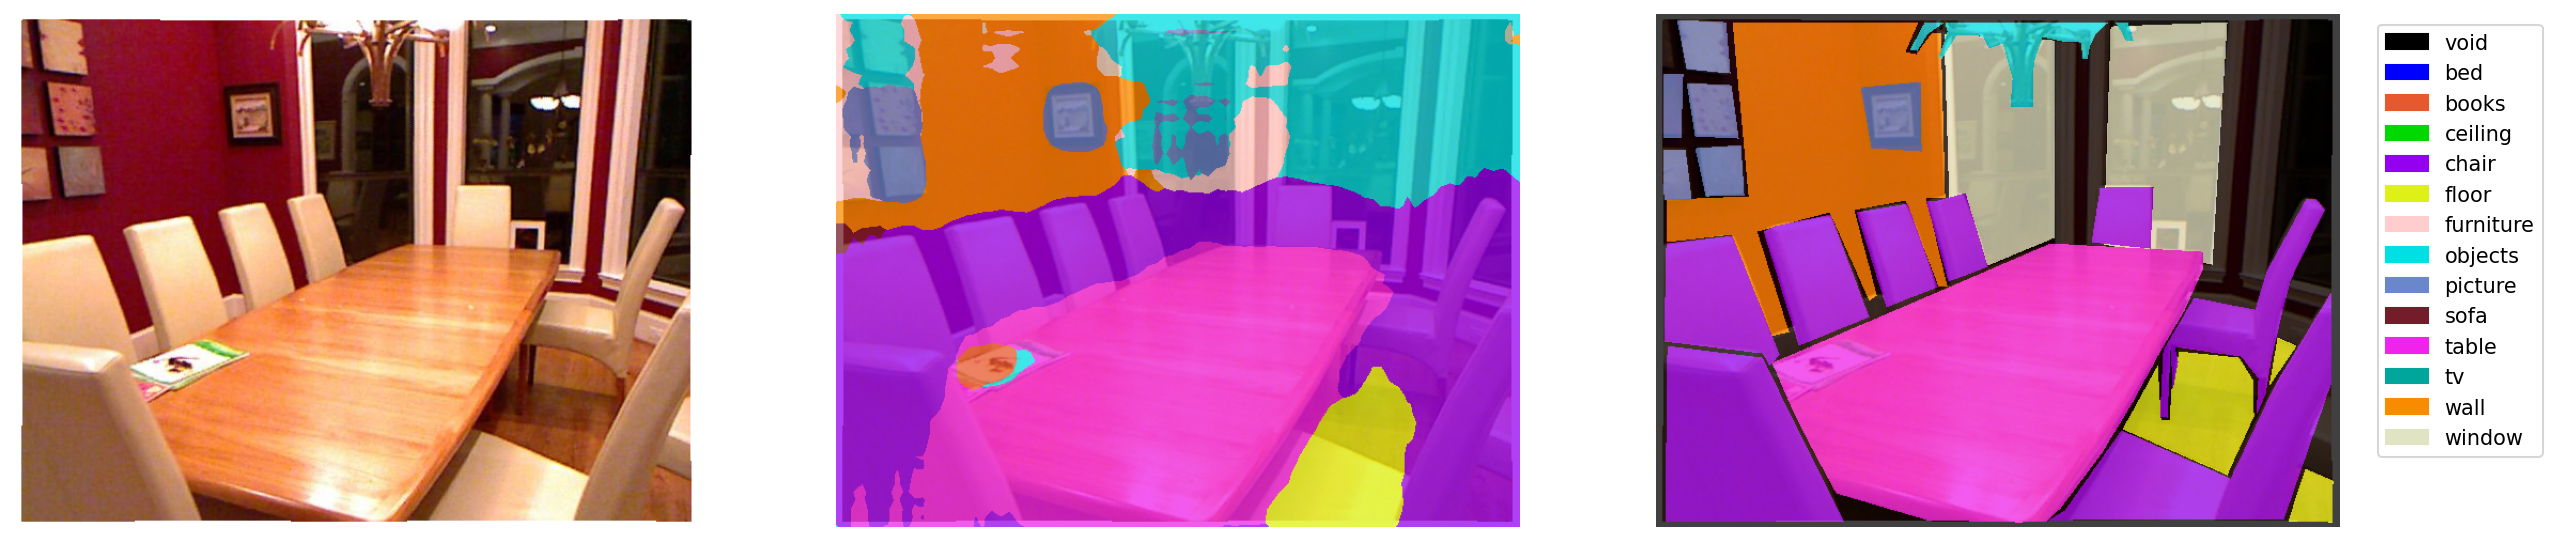
\includegraphics[width=\textwidth]{img/preds_analysis/gt_vs_pred/dining_room-2.png}
    \caption{Porównanie jakości segmentacji dla klasy jadalnia.}
    \label{fig:dining_room-pred-2}
\end{figure}

Ostanim analizowany obraz w jadalni jest rysunek \ref{fig:dining_room-pred-3}. Na pewno klasyfikacja klas takich jak stół, krzesła czy okno jest tutaj poprawna. Co więcej nie można tego do tego grona niezaliczyć klasy podłoga oraz sufit. Jedyny problem z grupowaniem na tym zdjęciu dotyczy samego roku zdjęcia, gdzie nie przyporządkowano klasy mebel. Pozostałe instacje tej klasy są poprawnie sklasyfikowane.

\begin{figure}[ht!]
    \centering
    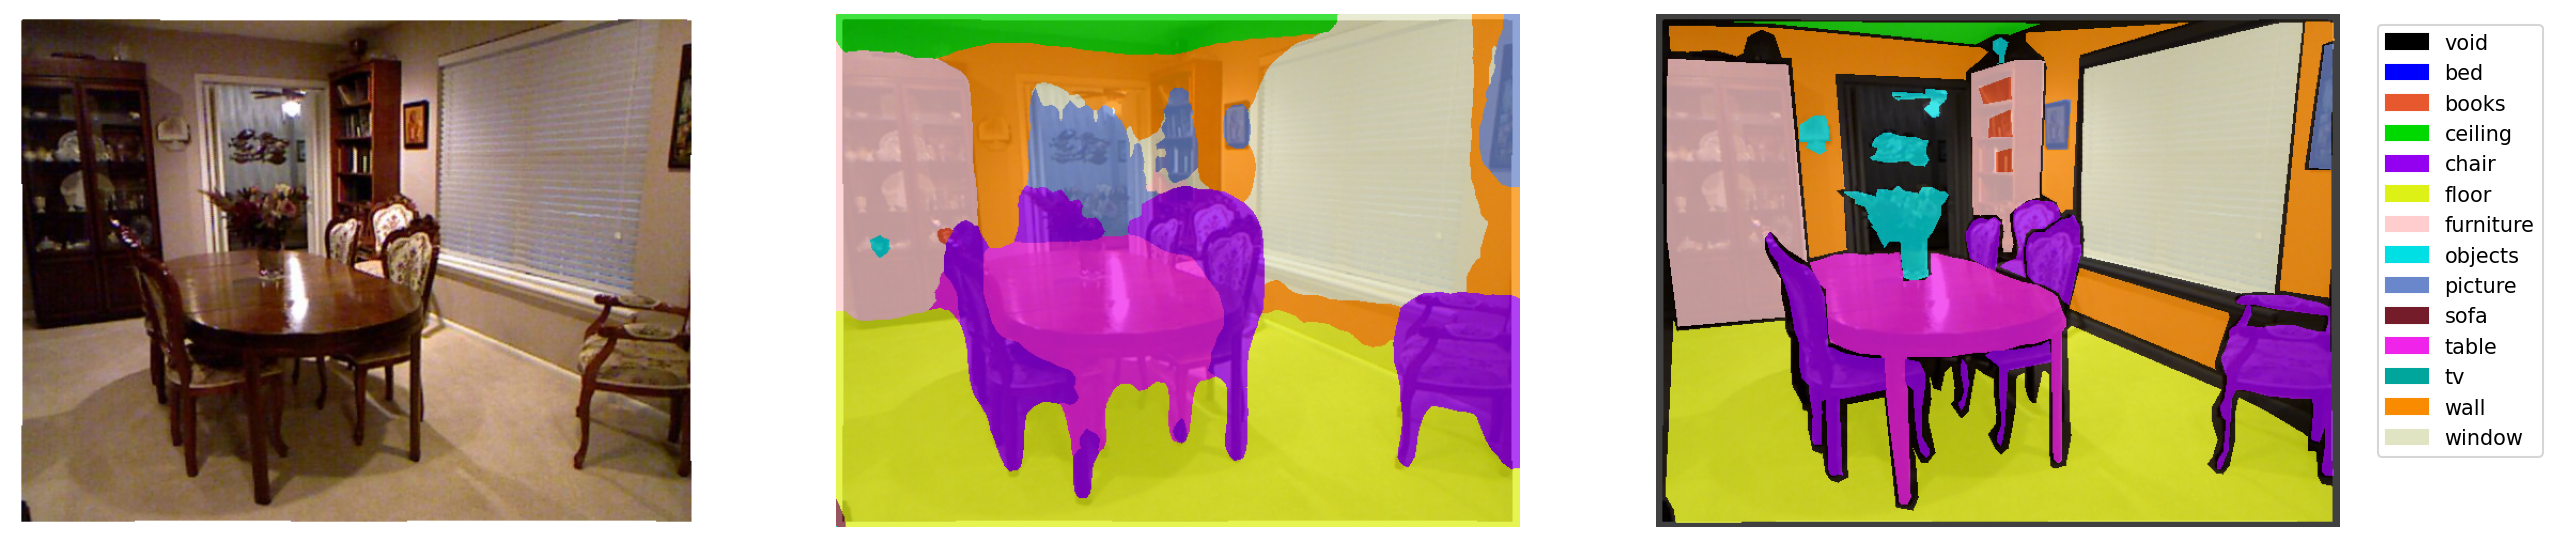
\includegraphics[width=\textwidth]{img/preds_analysis/gt_vs_pred/dining_room-3.png}
    \caption{Porównanie jakości segmentacji dla klasy jadalnia.}
    \label{fig:dining_room-pred-3}
\end{figure}

\noindent
\textbf{Kuchnia}

Obrazy przedstawiające kuchnie to głównie zabudowa kuchni oraz sprzęt kuchenny. Czasen występuje tutaj na przykład stół z krzesłami.

Obraz \ref{fig:kitchen-pred-1} nie wydaje się trudnym do klasyfikacji, jednak pojawiło się tutaj kilka kwestii ważnych omówienia. Oprócz problemów z klasyfikacją stołu z prawej strony, który bardziej wygląda jak szafki z blatem w kuchni, obserwujemy błędne przypisanie tapety naściennej jako obrazy. Poza tym drewniane drzwi model klasyfikuje jako bardziej mebel niż ścianę, co ze względu na teksturę nie jest aż tak złym wyborem. Reszta zdjęcia została pogrupowana poprawnie.

\begin{figure}[ht!]
    \centering
    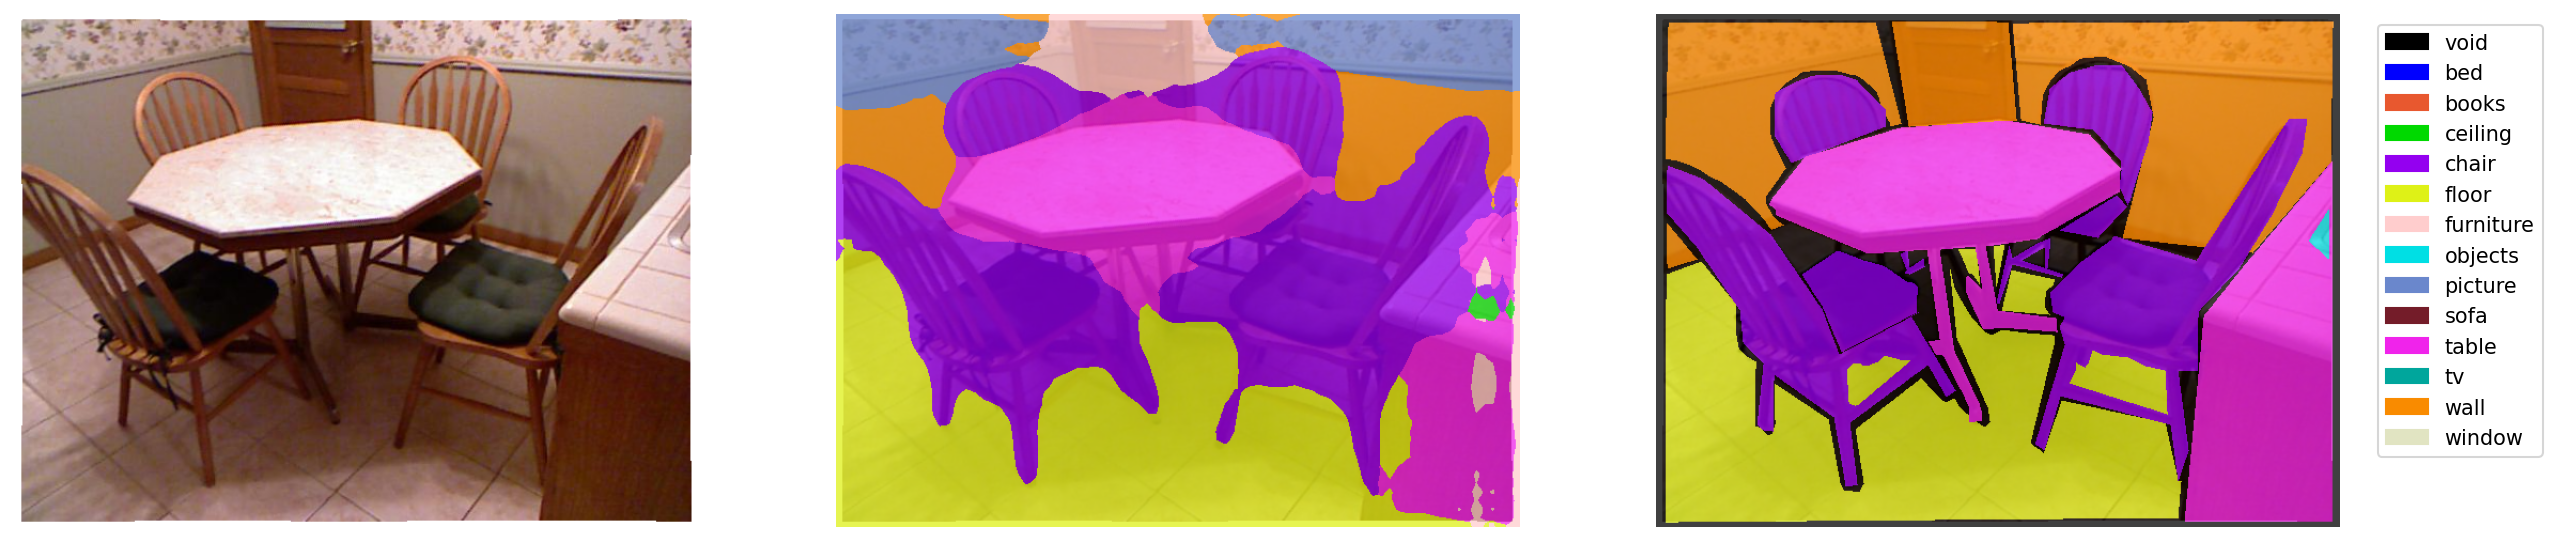
\includegraphics[width=\textwidth]{img/preds_analysis/gt_vs_pred/kitchen-1.png}
    \caption{Porównanie jakości segmentacji dla klasy kuchnia.}
    \label{fig:kitchen-pred-1}
\end{figure}

Na rysunku \ref{fig:kitchen-pred-2} widzimy typową wąską kuchnię. Rezultaty są w miarę zadowalające poza przypisaniem lodówki do klasy obraz. Prawdopodbnie miały na to wpływ zdjęcia zawieszone na lodówce. Ściany, szafki i sufit zostały zaklasyfikowany prawidłowo.

\begin{figure}[ht!]
    \centering
    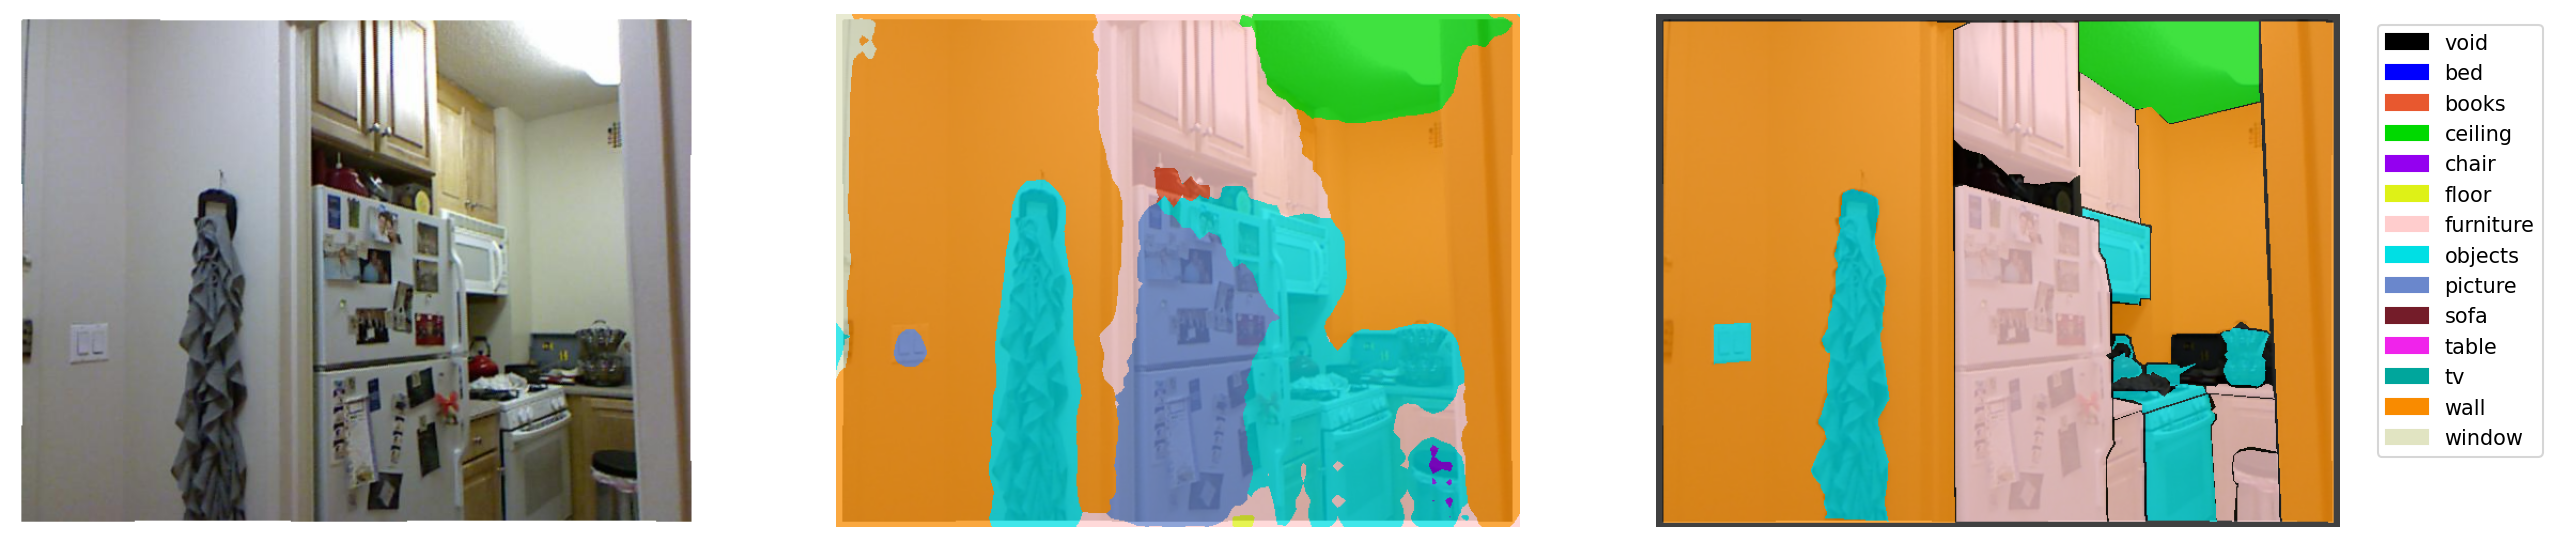
\includegraphics[width=\textwidth]{img/preds_analysis/gt_vs_pred/kitchen-2.png}
    \caption{Porównanie jakości segmentacji dla klasy kuchnia.}
    \label{fig:kitchen-pred-2}
\end{figure}

Trzecim rysunkiem jest rys. \ref{fig:kitchen-pred-3}. Największe wyzwanie stanowią tutaj obiekty zlokalizowane w różnych miejscach. Cieszy fakt, że mimo iż autorzy błędnie ocenili krzesło jako obiekt, model i tak zaznaczył je poprawnie. Widzimy tutaj również próbę klasyfikacji stołu. Powraca wtedy dyskusja na temat czy stół jest meblem tak jak został zaklasyfikowany przez model.

\begin{figure}[ht!]
    \centering
    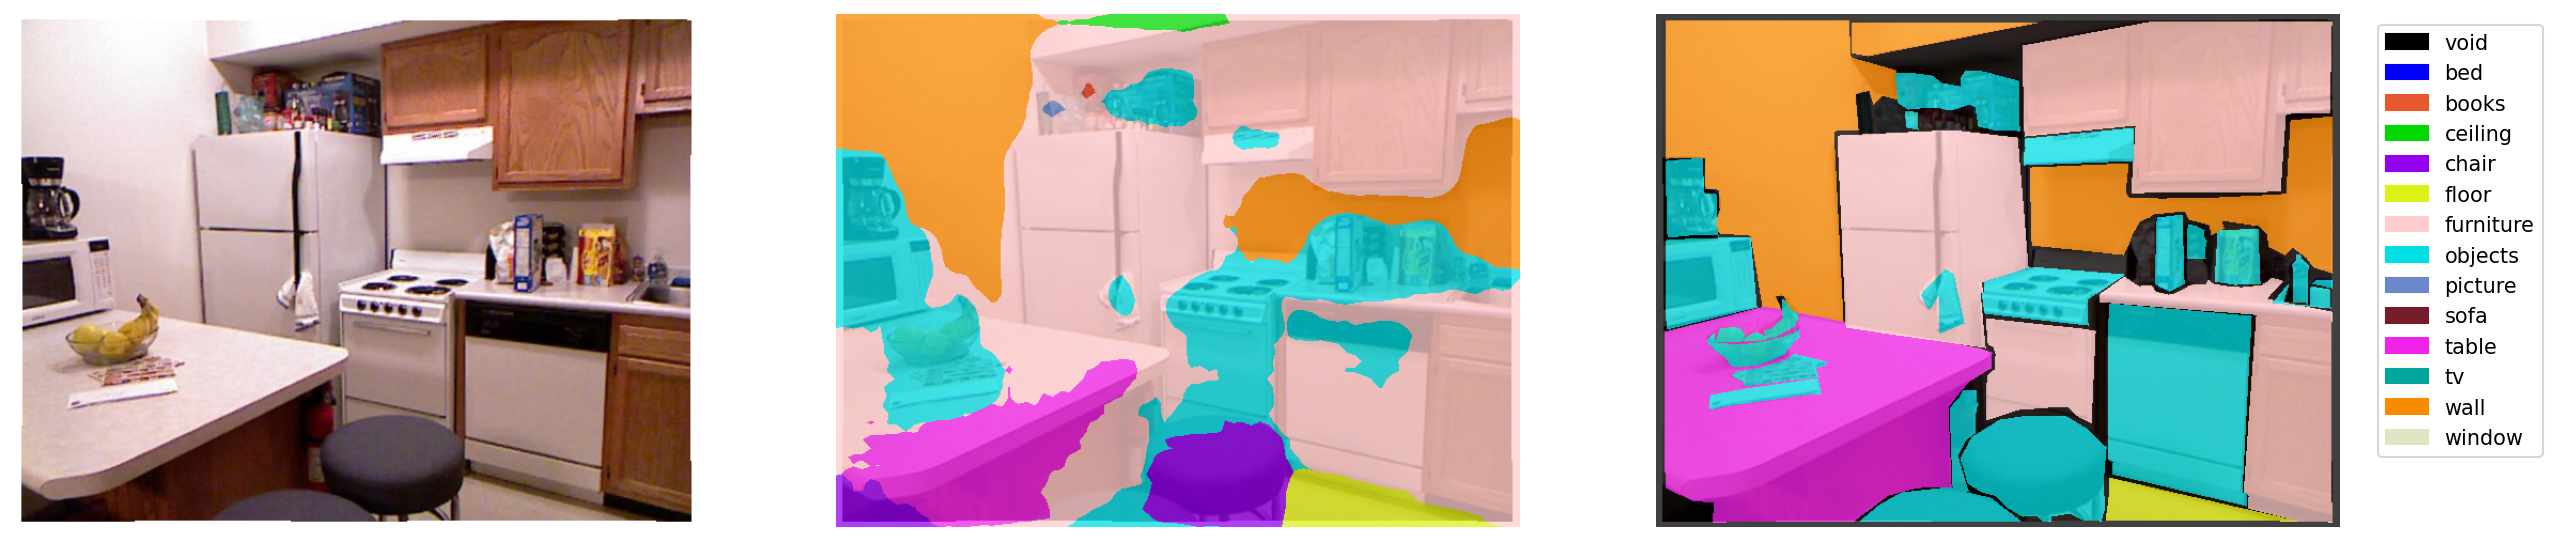
\includegraphics[width=\textwidth]{img/preds_analysis/gt_vs_pred/kitchen-3.png}
    \caption{Porównanie jakości segmentacji dla klasy kuchnia.}
    \label{fig:kitchen-pred-3}
\end{figure}

\noindent
\textbf{Biuro}

Sceny związane z biurem najczęściej przedstawiają biurka z krzesłami, zarówno w faktycznych biurach, o których często świadczy wykładzina, jak i w domowych pokojach typu biuro.

Na rysunku \ref{fig:office-pred-1} widać scenę przedstawiające pokój z drukarkami. Model dość dobrze radzi sobie ze ścianami oraz z podłogą, której akurat w tym przypadku nie ma zbyt wiele. Ciekawa jest wizja autorów zbioru danych określających mapę jako obiekt zamiast obraz. Może trudno bez wahania przypisać wiszącej mapie miano obrazu, ale na pewno szybciej możną ją określić jako plakat co można tłumazyć na angielski jako picture.

\begin{figure}[ht!]
    \centering
    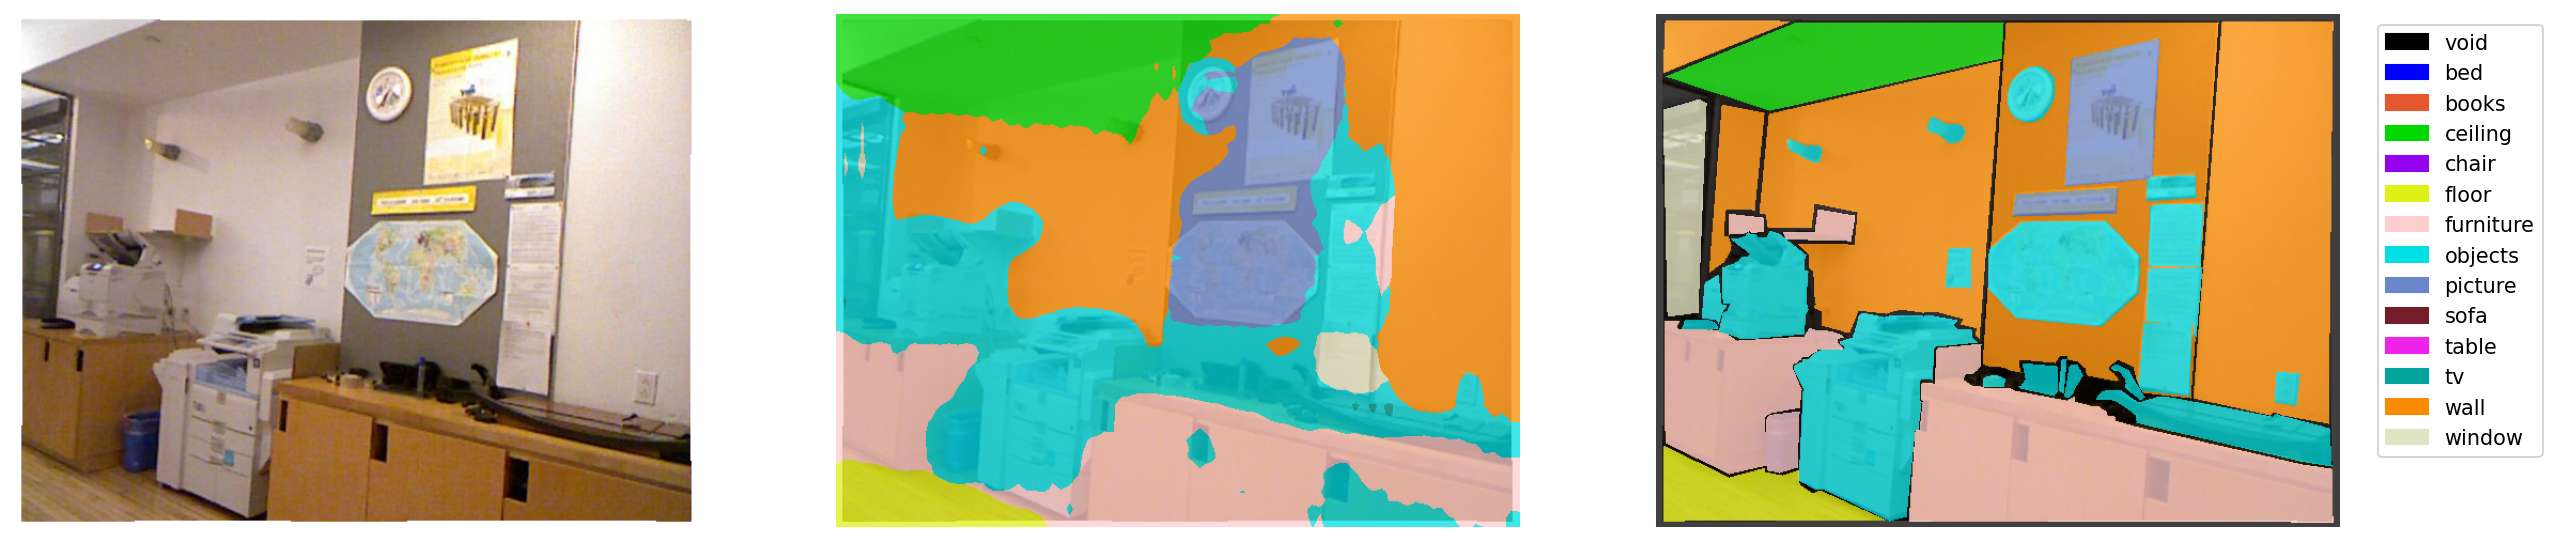
\includegraphics[width=\textwidth]{img/preds_analysis/gt_vs_pred/office-1.png}
    \caption{Porównanie jakości segmentacji dla klasy biuro.}
    \label{fig:office-pred-1}
\end{figure}

Rysunek \ref{fig:office-pred-2} przedstawia salę konferencyjną. Lewa strona obrazu została zaklasyfikowana całkiem poprawnie. Wyzwaniem dla modelu okazał się prawy dolny róg, gdzie należało przypisać klasy mebel, obiekt, ściana, co model uprościł do po prostu mebla. To zdecydowanie zła klasyfikacja.

\begin{figure}[ht!]
    \centering
    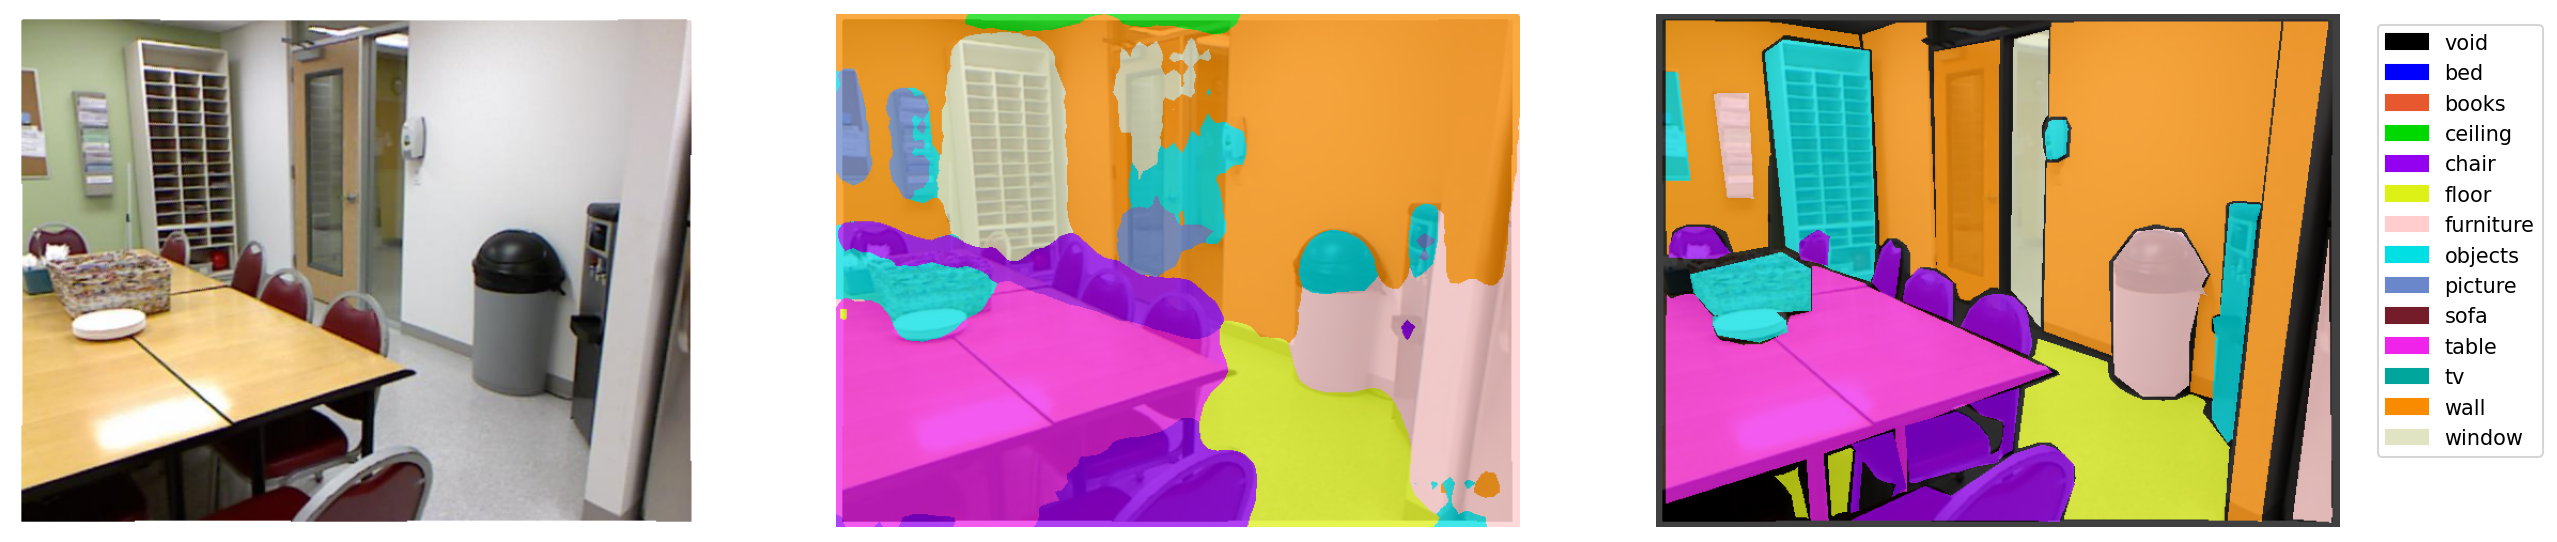
\includegraphics[width=\textwidth]{img/preds_analysis/gt_vs_pred/office-2.png}
    \caption{Porównanie jakości segmentacji dla klasy biuro.}
    \label{fig:office-pred-2}
\end{figure}

Ostanim rysunkiem {\ref{fig:office-pred-3}} jest pomiesczenie przedstawiające najprawdopodobniej biuro domowe. Klasyfikacja okna, podłogi oraz ściany była prawie bezbłędna. Gorzej model porawdził sobie z stołem, który po części sklasyfikował jako telewizor ze względu na bardzo ciemny oraz prostokąty charakter.

\begin{figure}[ht!]
    \centering
    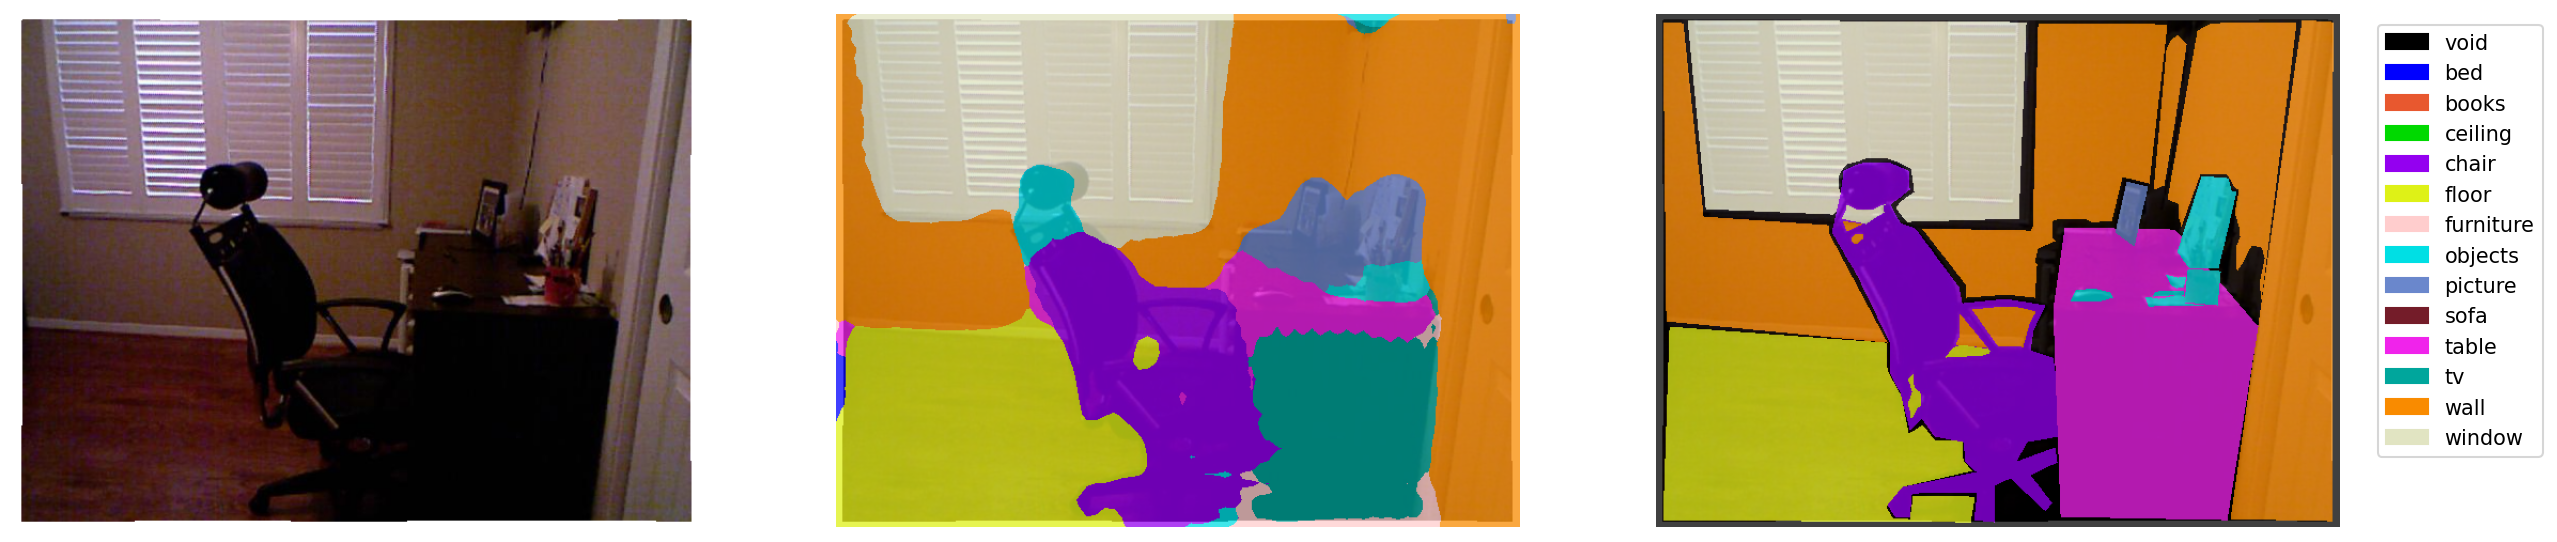
\includegraphics[width=\textwidth]{img/preds_analysis/gt_vs_pred/office-3.png}
    \caption{Porównanie jakości segmentacji dla klasy biuro.}
    \label{fig:office-pred-3}
\end{figure}

\noindent
\textbf{Inne pomieszczenia}

Sceny związane z klasą inne pomieszczenia budzą najwięcej wątplości. Nie wiadomo bowiem, co dokładnie może się tam znaleźć.

Na rysunku \ref{fig:other_indoor-pred-1} znajduje się wspólna przesztrzeń biurowa. Widzimy, że znajduje się tutaj wiele obszarów typu void, zatem model dokładnie nie wie co powinno się tam znaleźć. Dziwi to szczególnie w przypadku pierwszego krzesła po prawej stronie. Nie mniej jednak model dość dobrze zgaduję tę klasę. Jest zrozumiałym, że pokój otoczy ścianami. W gruncie rzeczy szklana szyba rzeczywiście jest ścianą w tym przypadku. Model niezbyt dobrze pogrupował klasę obiekty. Jest tutaj wiele do poprawy.

\begin{figure}[ht!]
    \centering
    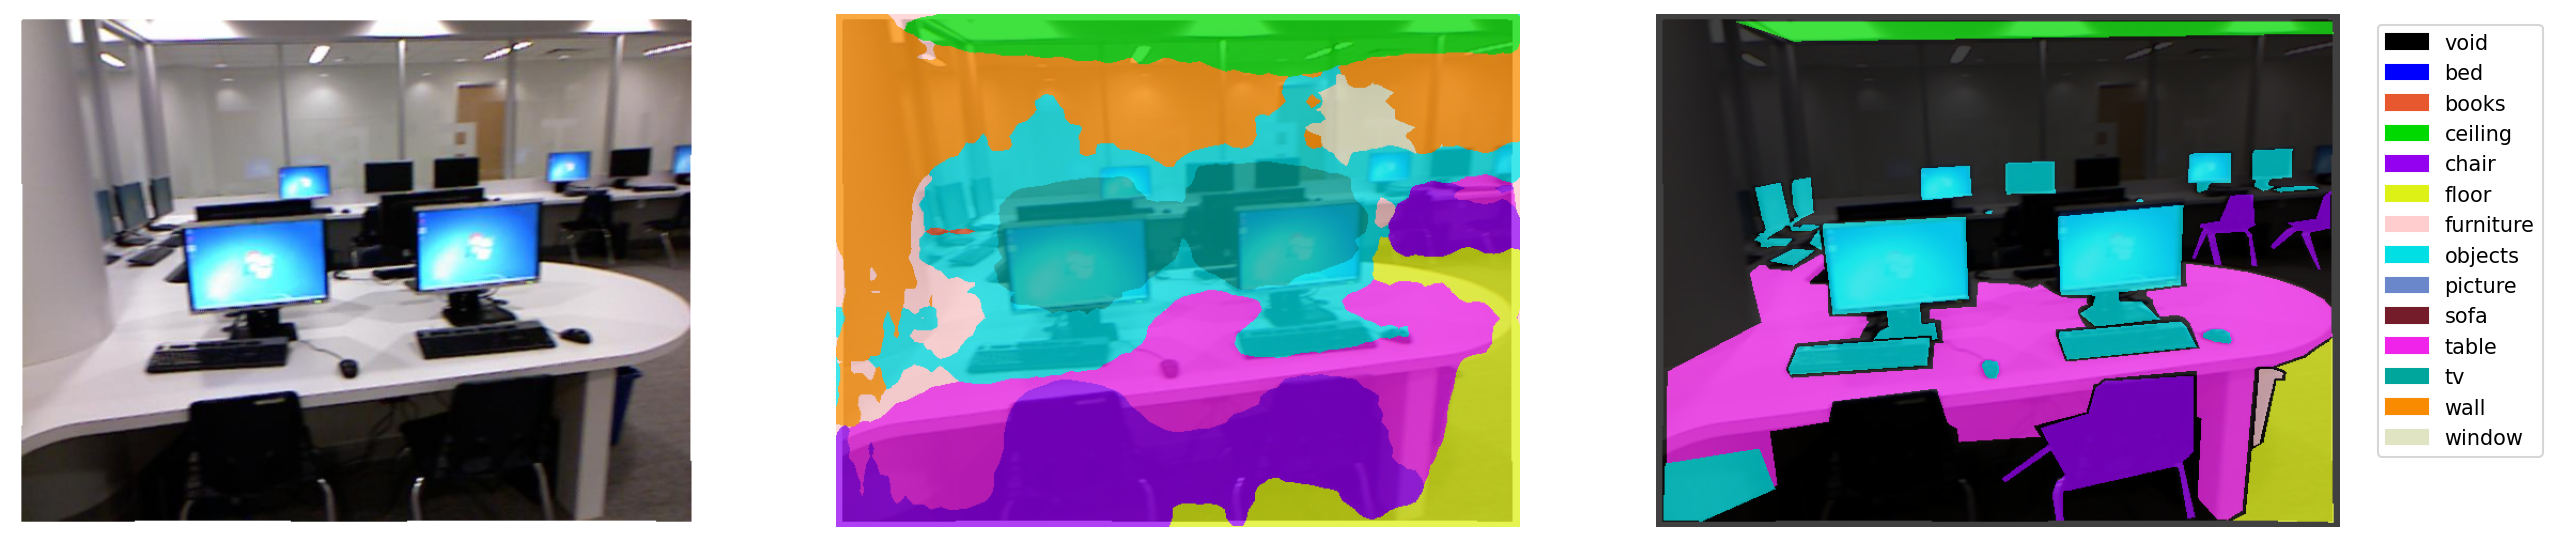
\includegraphics[width=\textwidth]{img/preds_analysis/gt_vs_pred/other_indoor-1.png}
    \caption{Porównanie jakości segmentacji dla klasy inne pomieszczenia.}
    \label{fig:other_indoor-pred-1}
\end{figure}

Rysunek \ref{fig:other_indoor-pred-2} przedstawia pomieszczenie biurowe. Wszystkie obrazki zostały zaklasyfikowane poprawnie. Okna zostały przypisane jako obrazy. Model dobrze pogrupował człowieka. Wyzwanie stanowiła klasa obiekty.

\begin{figure}[ht!]
    \centering
    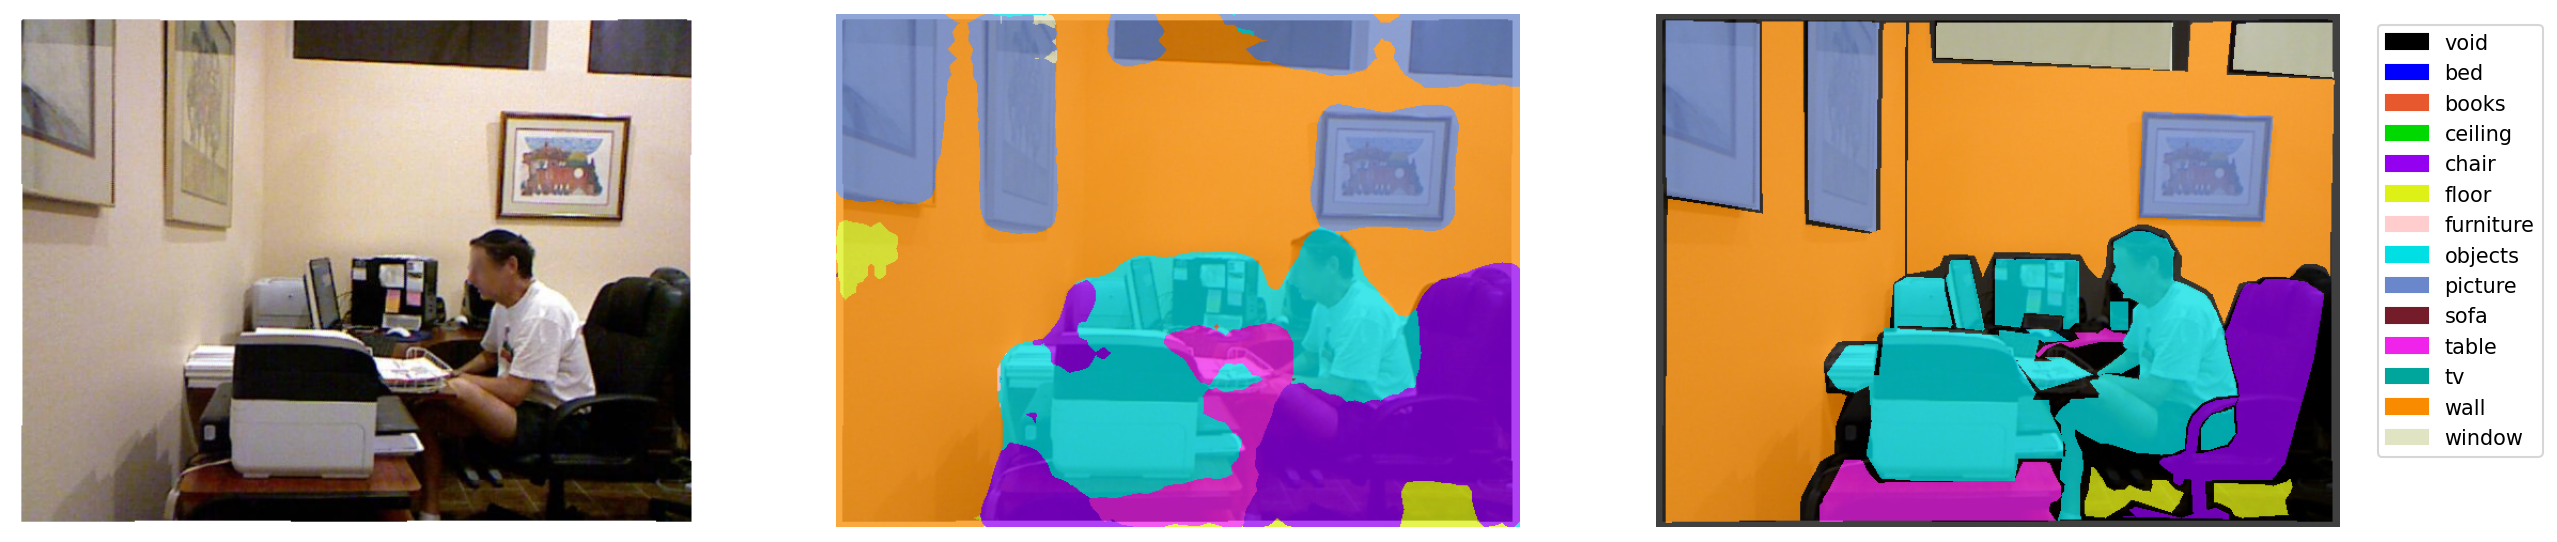
\includegraphics[width=\textwidth]{img/preds_analysis/gt_vs_pred/other_indoor-2.png}
    \caption{Porównanie jakości segmentacji dla klasy inne pomieszczenia.}
    \label{fig:other_indoor-pred-2}
\end{figure}


Ostatnim analizowanym obrazem w jadalni jest rysunek \ref{fig:dining_room-pred-3}. Na pewno klasyfikacja stółu, krzesła czy okna jest tutaj poprawna. Co więcej, nie można tego do tego grona nie zaliczyć klasy podłoga oraz sufit. Jedyny problem z grupowaniem na tym zdjęciu dotyczy samego rogu zdjęcia, gdzie nie przyporządkowano klasy mebel. Pozostałe instancje tej klasy są poprawnie sklasyfikowane.

\begin{figure}[ht!]
    \centering
    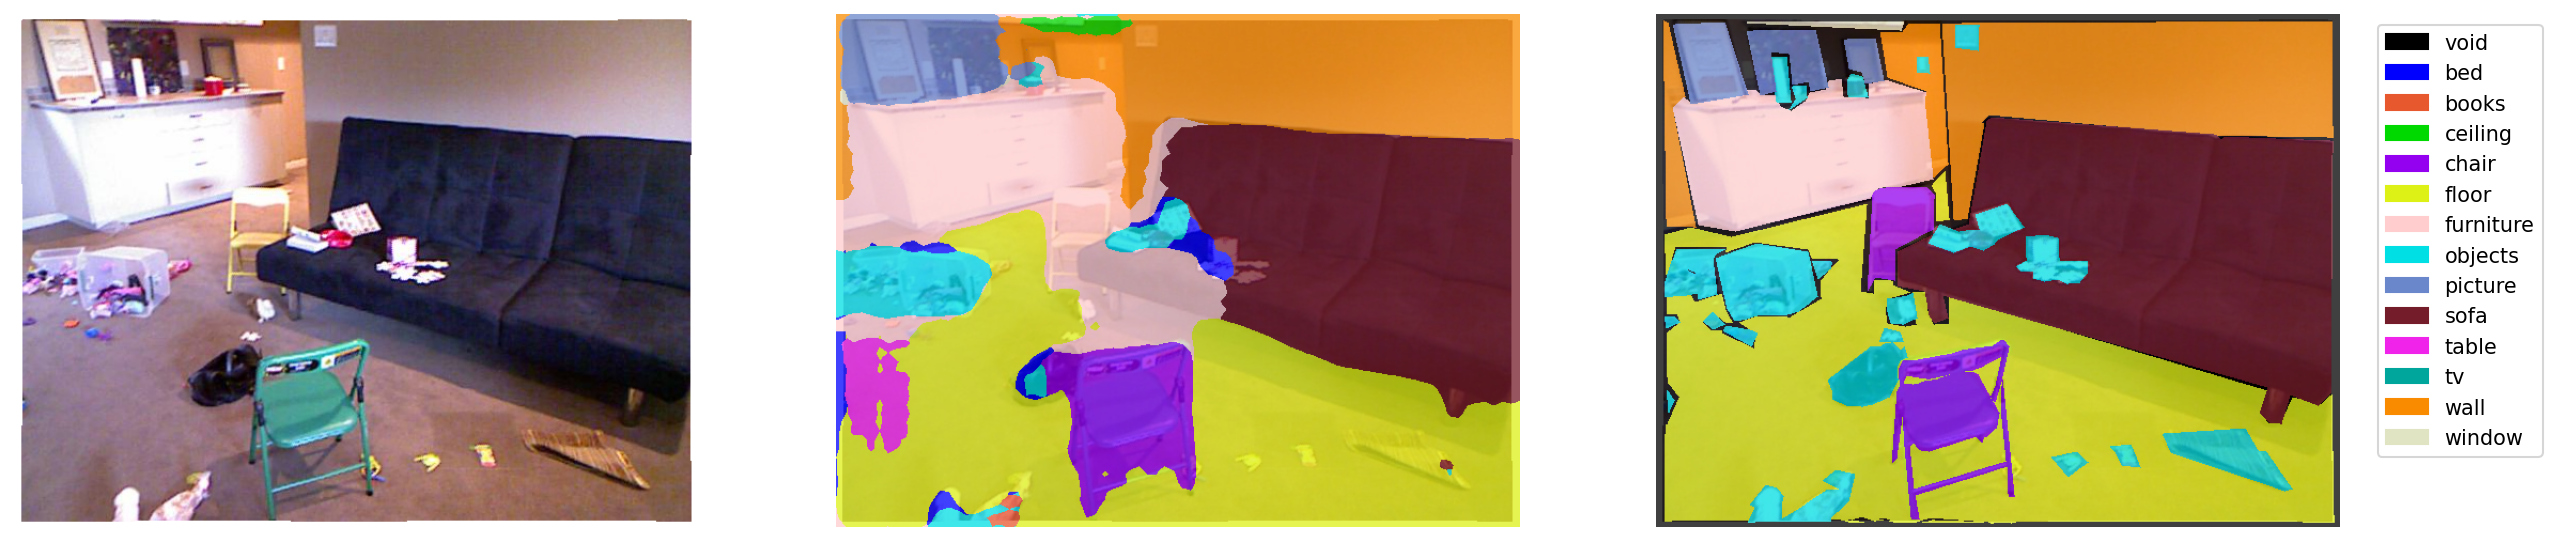
\includegraphics[width=\textwidth]{img/preds_analysis/gt_vs_pred/other_indoor-3.png}
    \caption{Porównanie jakości segmentacji dla klasy inne pomieszczenia.}
    \label{fig:other_indoor-pred-3}
\end{figure}

\subsubsection{Klasyfikacja sceny}
Podobnie jak w przypadku segmentacji semantycznej czasem trudno jest jednoznacznie określić jakość modelu, bazując wyłącznie na miarach jakości. W niniejszym rozdziale zostaną przytoczone wszystkie błędne klasyfikacje z podziałem na konkretne klasy. Pozwoli to wysnuć pewne obserwacje na temat podobieństw tych klas oraz pomoże wysunąć wnioski co do tych błędów. Co więcej, przedstawione zostaną statystyki błędnej klasyfikacji, aby lepiej zobrazować te błędy.

Na rysunku \ref{fig:bathroom-false-pred} przedstawiono 10 błędnych przypisań dla klasy łazienka. Dziewięć z dziesięciu błędów dotyczyło klasy kuchnia. Można doszukiwać się, że kuchnia, jak i łazienka ma poniekąd podobny schemat. Na pewno występuję te same klasy jak zlew czy meble. Tylko raz klasyfikator uznał, że sypialnia jest łazienką.
\begin{figure}[ht!]
    \centering
    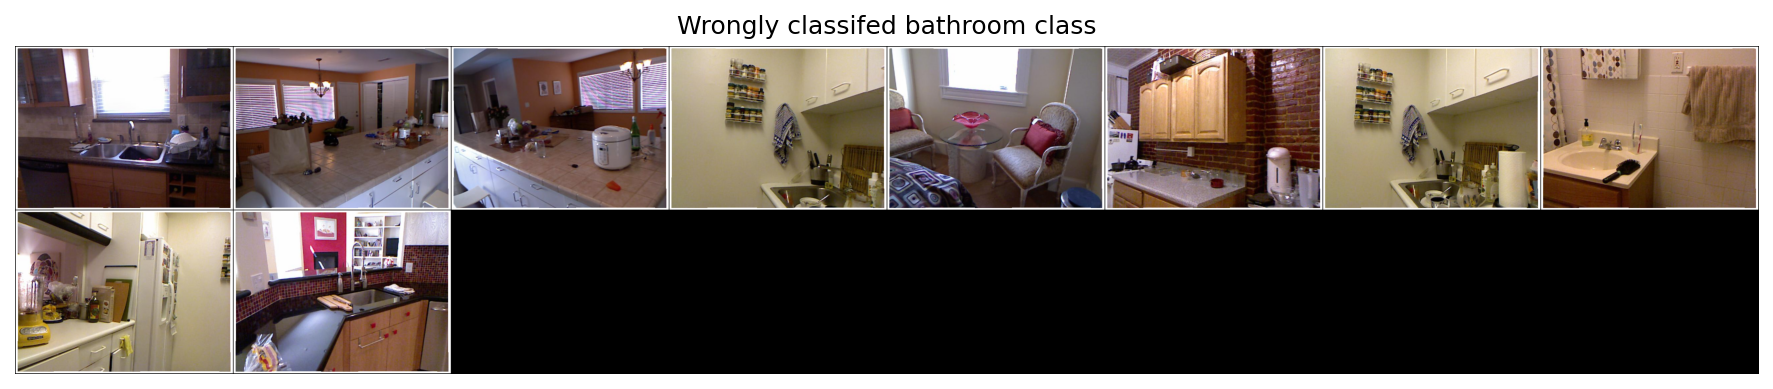
\includegraphics[width=\textwidth]{img/preds_analysis/classification/bathroom.png}
    \caption{Porównanie jakości klasyfikacji dla klasy łazienka.}
    \label{fig:bathroom-false-pred}
\end{figure}
Najwięcej pomyłek algorytm popełnił na klasie sypialnia (rys.\ref{fig:bedroom-false-pred}). Na pewno wynika to z faktu, iż była to klasa dominująca. Co drugi błąd następował na klasie sypialnia. Szczególnie często gdy łózkiem była kanapa lub na zdjęiu występował fotel. Ponad 32\% błędów w sumie stanowiły klasy biuro oraz jadalnia. Można przypuszczać, że tym razem kluczowym elementem świadczącym o predykcji był stół.
\begin{figure}[ht!]
    \centering
    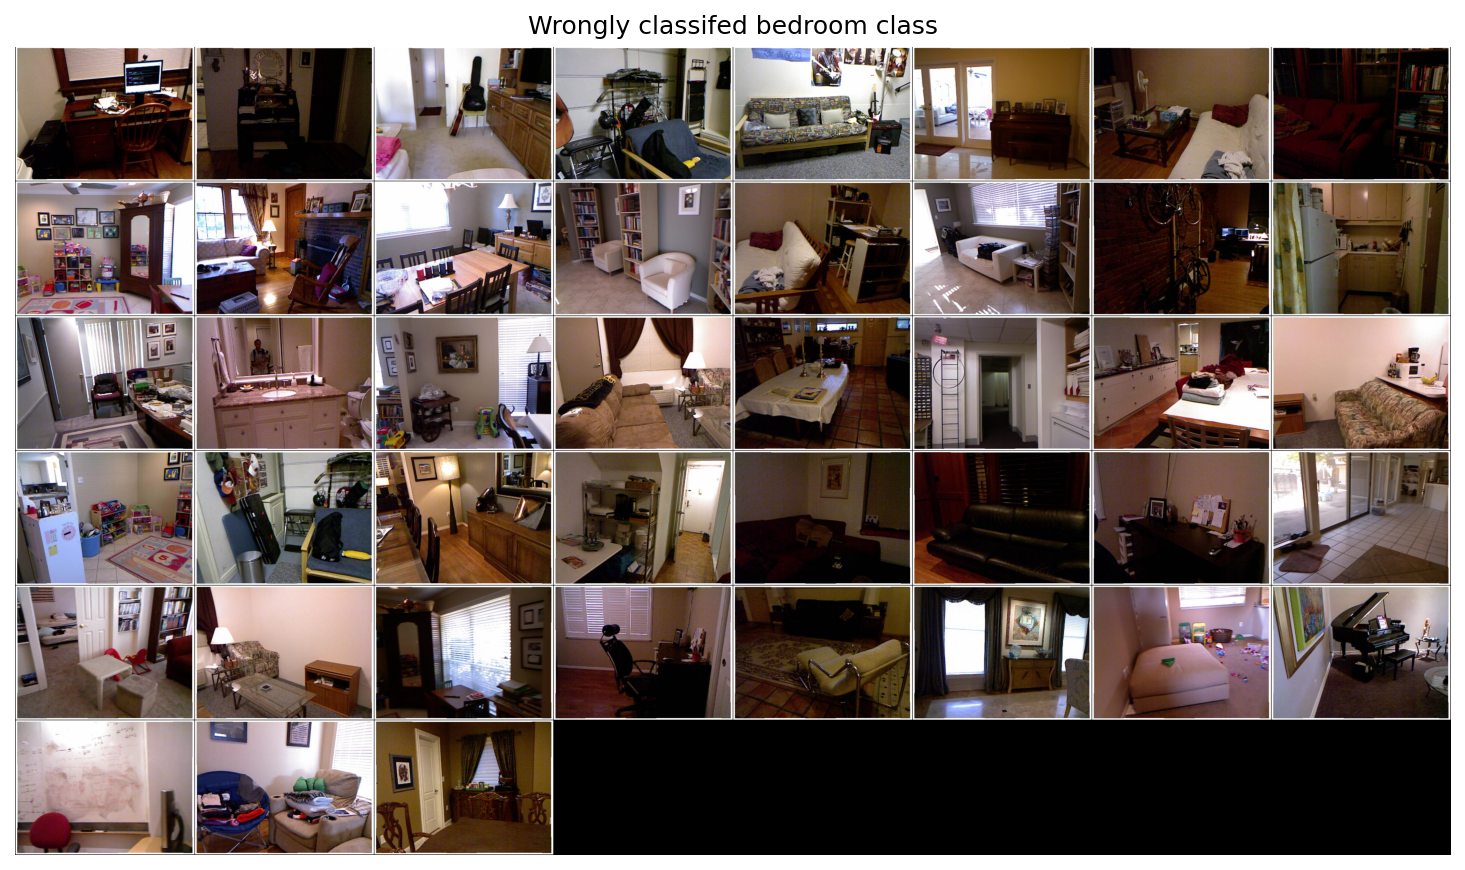
\includegraphics[width=\textwidth]{img/preds_analysis/classification/bedroom.png}
    \caption{Porównanie jakości klasyfikacji dla klasy sypialnia.}
    \label{fig:bedroom-false-pred}
\end{figure}
Jadalnia była pomylona w sumie 11 razy (rys. \ref{fig:dining_room-false-pred}). Zgodnie z przedstawionym rysunkiem, na większości zdjęć występuje stół i krzesła.

\begin{figure}[ht!]
    \centering
    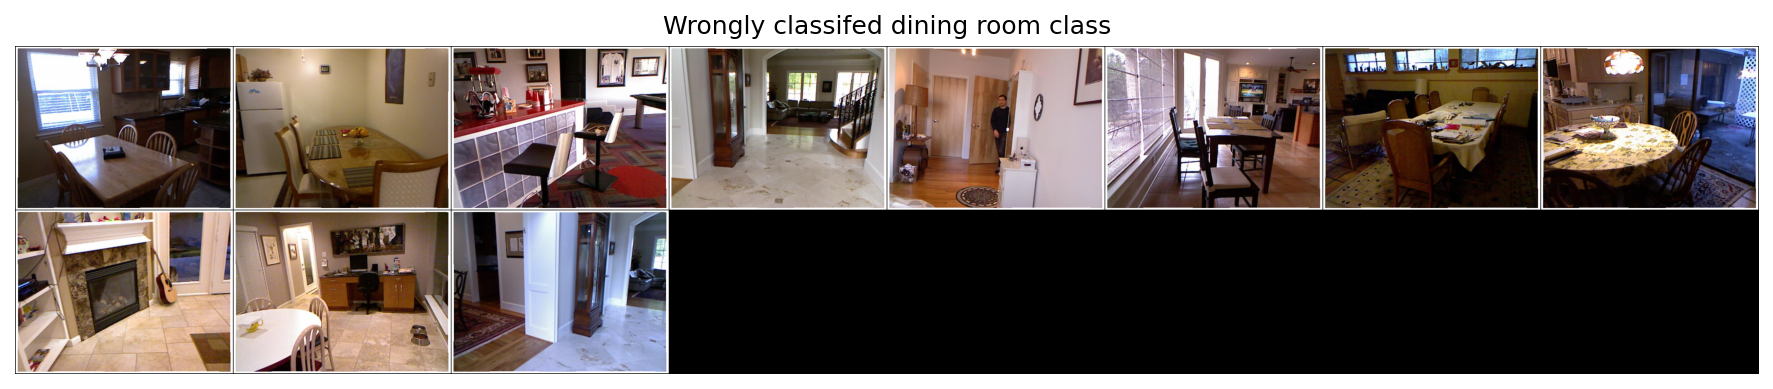
\includegraphics[width=\textwidth]{img/preds_analysis/classification/dining_room.png}
    \caption{Porównanie jakości klasyfikacji dla klasy jadalnia.}
    \label{fig:dining_room-false-pred}
\end{figure}
Najmniej pomyłek jest dla klasy kuchnia (rys. \ref{fig:kitchen-false-pred}).
\begin{figure}[ht!]
    \centering
    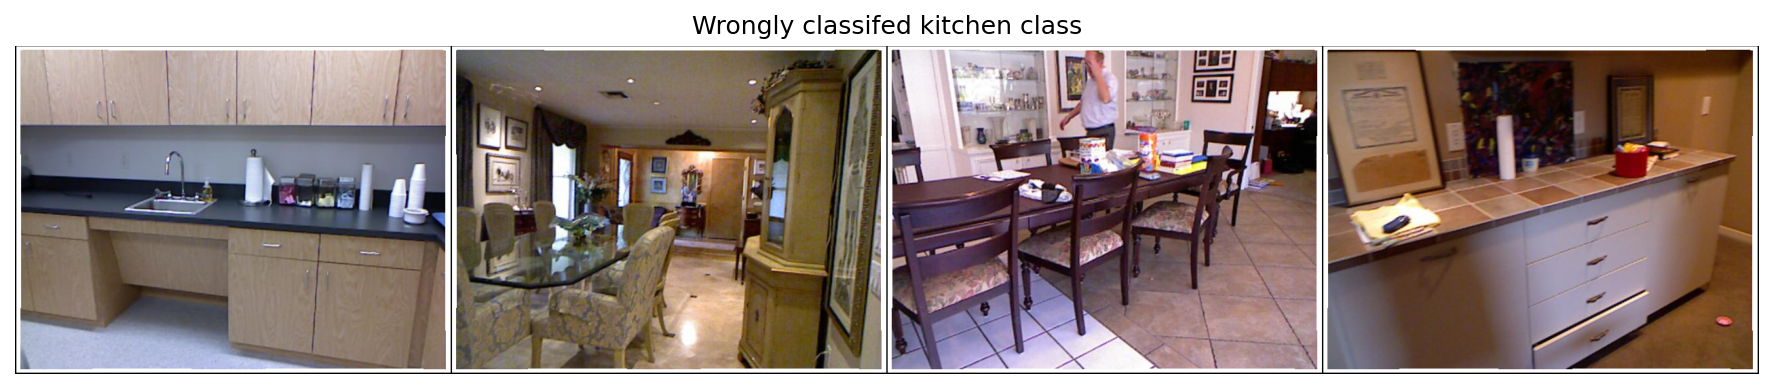
\includegraphics[width=\textwidth]{img/preds_analysis/classification/kitchen.png}
    \caption{Porównanie jakości klasyfikacji dla klasy kuchnia.}
    \label{fig:kitchen-false-pred}
\end{figure}
Klasy inne pomieszczenia oraz kuchnie zostały błędnie zaklasyfikowane jako biuro w większości przypadków. Trudno określić, skąd akurat wynikają takie rezultaty.

\begin{figure}[ht!]
    \centering
    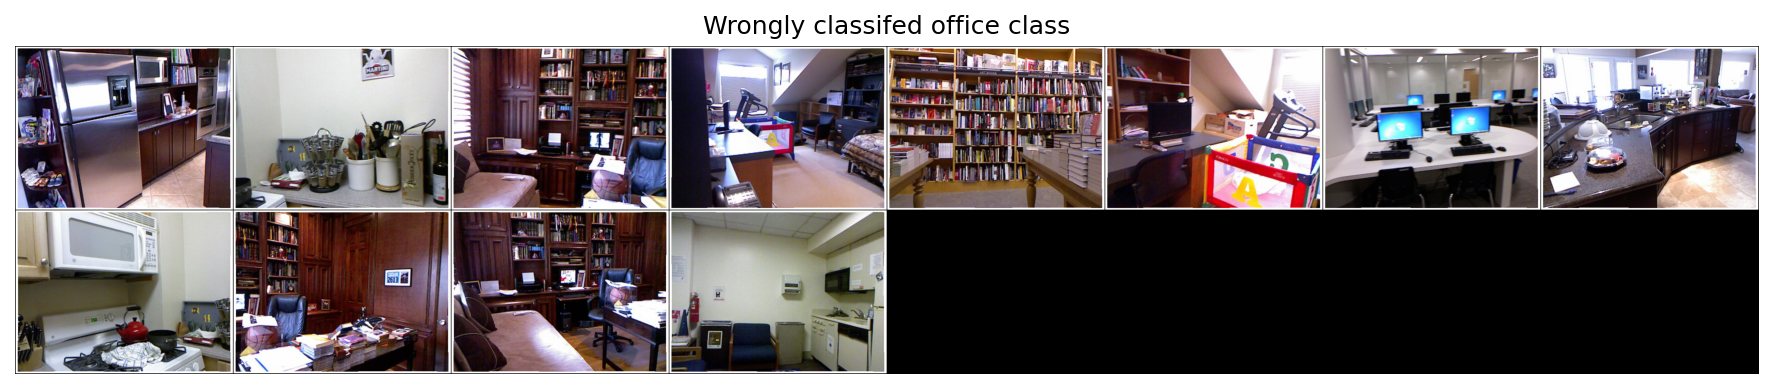
\includegraphics[width=\textwidth]{img/preds_analysis/classification/office.png}
    \caption{Porównanie jakości klasyfikacji dla klasy biuro.}
    \label{fig:office-false-pred}
\end{figure}
Model najczęściej błędnie przypisywał klasę inne pomieszczenia dla biura w mniej niż połowie przypadków. Pozostałe przypadki należą do klas sypialnia oraz jadalnia. Klasa inne pomieszczenia jest szczególnie narażona na pomyłki, gdyż to połączenie najróżniejszych klas scen.
\begin{figure}[ht!]
    \centering
    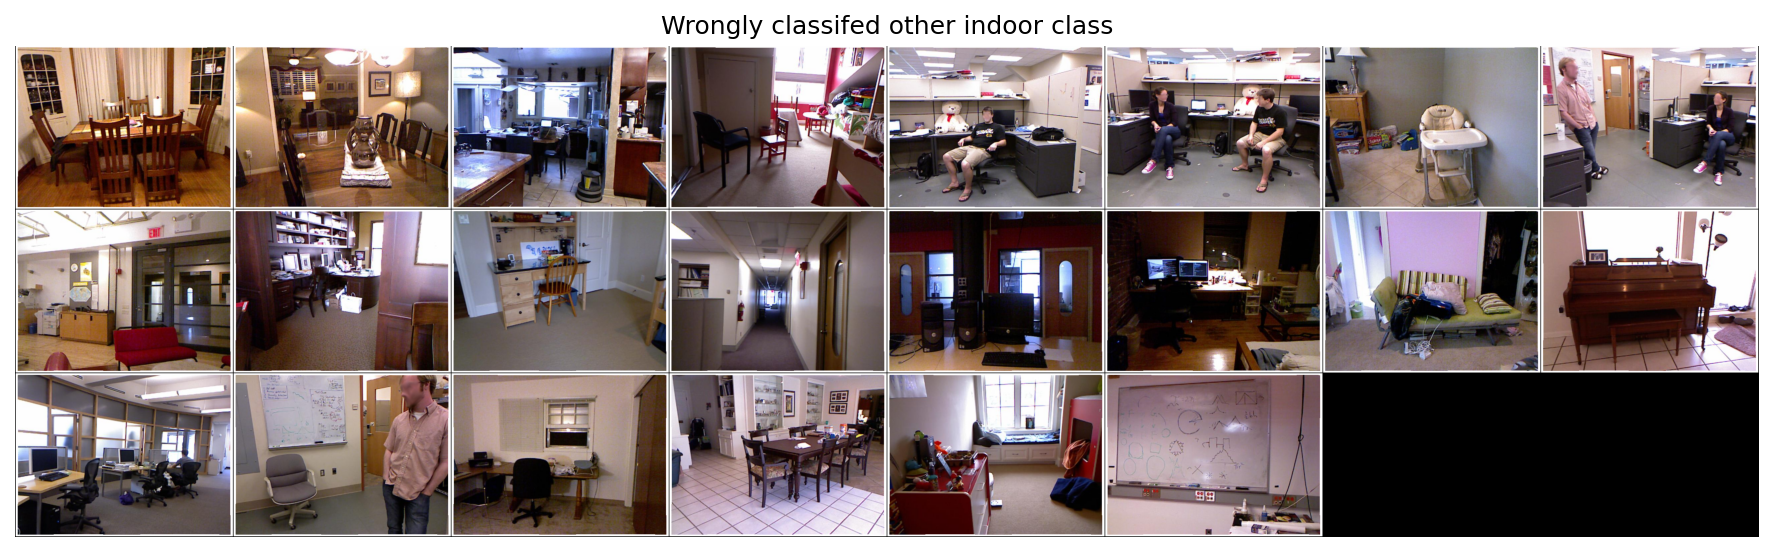
\includegraphics[width=\textwidth]{img/preds_analysis/classification/other_indoor.png}
    \caption{Porównanie jakości klasyfikacji dla klasy inne pomieszczenia.}
    \label{fig:oter_indoor-false-pred}
\end{figure}


Analiza błędnie sklasyfikowany scen dostarczyła wielu ważnych informacji. Najczęściej przyczyną błędów było znaczne podobieństwo występujących klas przedmiotów między różnymi klasami scen.


    
    % \begin{figure}[ht!]
    %     \centering
    %     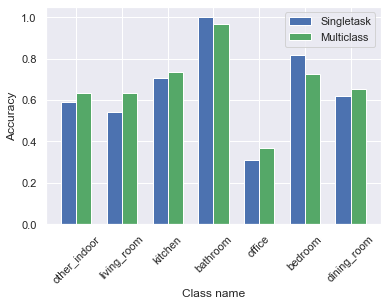
\includegraphics[width=0.75\textwidth]{scene_comp.png}
    %     \caption{Porównanie dokładności dla każdej z klas w zadaniu klasyfikacji pomieszczeń}
    %     \label{fig:scene_comp}
    % \end{figure}
    
    % \begin{figure}[ht!]
    %     \centering
    %     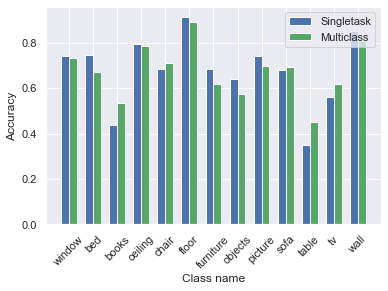
\includegraphics[width=0.75\textwidth]{seg_comp.png}
    %     \caption{Porównanie dokładności dla każdej z klas w zadaniu segmentacji semantycznej}
    %     \label{fig:seg_comp}
    % \end{figure}
    % Ucznie wielozadaniowe w rozważanym przypadku nieznacznie poprawia wyniki sieci (tab. \ref{tab:acc-por}). Dla zadania segmentacji semantycznej otrzymujemy spadek jakości o 0.39 punkta procentowego. Zadanie klasyfikacji poprawia się o 1.95 p.p. w porównaniu z uczeniem jednozadaniowym. Ostatecznie otrzymujemy zysk na poziomie 0.78 punkta procentego na średniej z zadań. Poprawa jest niewielka, jednak jest to dużu sukces biorąc pod uwagę, że mamy do dyspozycji 2 razy mniej parametrów niz w przypadku dwóch osobnych sieci. Przekłada się to bezpośrednio na czas inferencji, który w przypadku robotyki i systemów czasu rzeczywistego jest kluczowy.
    
    % Wartym zobaczenia jest fakt, iż uczenie wielozadaniowe poprawia wyniki dla klas które osiągają najsłabsze rezultaty w uczeniu jednozadaniowym. Poprawie ulega klasa office (rys. \ref{fig:scene_comp}) dla klasyfikacji oraz klasy books oraz table (rys. \ref{fig:seg_comp}) dla segmentacji semantycznej. Powodem jest prawdopodbnie mniejsze obciążenie (bias) modelu spowodowane faktem wzajemnej regularyzacji obu zadań w procesie uczenia. Innymi słowy, model ma mniejszą tendencję do przeuczenia.